% mnras_template.tex
%
% LaTeX template for creating an MNRAS paper
%
% v3.0 released 14 May 2015
% (version numbers match those of mnras.cls)
%
% Copyright (C) Royal Astronomical Society 2015
% Authors:
% Keith T. Smith (Royal Astronomical Society)

% Change log
%
% v3.0 May 2015
%    Renamed to match the new package name
%    Version number matches mnras.cls
%    A few minor tweaks to wording
% v1.0 September 2013
%    Beta testing only - never publicly released
%    First version: a simple (ish) template for creating an MNRAS paper

%%%%%%%%%%%%%%%%%%%%%%%%%%%%%%%%%%%%%%%%%%%%%%%%%%
% Basic setup. Most papers should leave these options alone.
\documentclass[a4paper,fleqn,usenatbib,letter]{mnras}

% MNRAS is set in Times font. If you don't have this installed (most LaTeX
% installations will be fine) or prefer the old Computer Modern fonts, comment
% out the following line
\usepackage{newtxtext,newtxmath}
% Depending on your LaTeX fonts installation, you might get better results with one of these:
%\usepackage{mathptmx}
%\usepackage{txfonts}

% Use vector fonts, so it zooms properly in on-screen viewing software
% Don't change these lines unless you know what you are doing
\usepackage[T1]{fontenc}
\usepackage{ae,aecompl}


%%%%% AUTHORS - PLACE YOUR OWN PACKAGES HERE %%%%%

% Only include extra packages if you really need them. Common packages are:
\usepackage{graphicx}	% Including figure files
\usepackage{amsmath}	% Advanced maths commands
\usepackage{amssymb}	% Extra maths symbols

%%%%%%%%%%%%%%%%%%%%%%%%%%%%%%%%%%%%%%%%%%%%%%%%%%

%%%%% AUTHORS - PLACE YOUR OWN COMMANDS HERE %%%%%

% Please keep new commands to a minimum, and use \newcommand not \def to avoid
% overwriting existing commands. Example:
%\newcommand{\pcm}{\,cm$^{-2}$}	% per cm-squared
\newcommand{\be}{\begin{equation}}
\newcommand{\ee}{\end{equation}} 
\newcommand{\bse}{\begin{subequations}}
\newcommand{\ese}{\end{subequations}} 
\newcommand{\bary}{\begin{eqnarray}}
\newcommand{\eary}{\end{eqnarray}} 
\newcommand{\di }{{\rm d}} 
\newcommand{\epsf}{\rm \epsilon_{\rm f}}
\newcommand{\epsr}{\rm \epsilon_{\rm r}}
\newcommand{\mbh}{ M_{\rm BH}}
%\newcommand{\mhalo}{\rm M_{\rm halo}}
\newcommand{\ms}{m_\ast}
\newcommand{\Lratio}{\rm log_{10}( \sigma_{500}/ L_{\rm aver,500})} 

\newcommand{\mdotbh}{\dot{M}_{\rm BH}} 
\newcommand{\mdoth}{\dot{\m}_{\rm halo}}
\newcommand{\mdots}{\dot{m}_\ast} 
\newcommand{\Msun}{\rm M_{\sun}}
\newcommand{\mseed}{m_{\rm seed}} 
\newcommand{\mdotbondi}{\dot{M}_{\rm Bondi}} 
\newcommand{\mdotedd}{\dot{M}_{\rm Edd}} 
\newcommand{\mstar}{M_{\rm star}}
\newcommand{\K}{\rm K}
\newcommand{\Vphi}{V_{\rm \phi}}
\newcommand{\cs}{ c_{\rm s}}
\newcommand{\Cvisc}{ C_{\rm visc}}
\newcommand{\mcrit}{ M_{200}}
\newcommand{\dNdLhx}{ \frac{{\rm d} N}{{\rm d} \log_{10} L_{HX} }}
\newcommand{\Ledd}{\lambda_{\rm Edd}}
\newcommand{\LhX}{L_{\rm HX}}
\newcommand{\Lbol}{L_{\rm bol}}
\newcommand{\ergs}{\mbox{erg}~\mbox{s}^{-1}}
\newcommand{\kpc}{\rm kpc}
\newcommand{\ckpc}{\rm ckpc}
\newcommand{\pkpc}{\rm pkpc}
\newcommand{\cMpc}{\rm cMpc}
\newcommand{\pMpc}{\rm pMpc}
\newcommand{\Mpc}{\rm Mpc}
\newcommand{\erg}{\rm erg}
\newcommand{\lsim}{\mathrel{\hbox{\rlap{\lower.55ex\hbox{$\sim$}} \kern-.3em\raise.4ex\hbox{$<$}}}}
\newcommand{\gsim}{\mathrel{\hbox{\rlap{\lower.55ex\hbox{$\sim$}} \kern-.3em\raise.4ex\hbox{$>$}}}}
\newcommand{\Lmaxb}{L_{\rm max,500,b} }
\newcommand{\Lmaxf}{L_{\rm max,500,f} }
\newcommand{\Laver}{L_{\rm aver,500} }
\newcommand{\REF}{Ref-L100N1504}
\newcommand{\REFSMALLMASS}{Ref-L100N0752}
\newcommand{\REFFIFTY}{Ref-L050N0752}
\newcommand{\AGNdT}{AGNdT9-L050N0752}
\newcommand{\RECAL}{Recal-L025N0752}
\newcommand{\SmallSeeds}{Small-seeds-L050N0752}
\newcommand{\Lmaxh}{L_{\rm max,500,h} }
\newcommand{\Lmaxl}{L_{\rm max,500,l} }
\newcommand{\Lmax}{L_{\rm max,500} }
\defcitealias{schaye2015}{S15}
\defcitealias{crain2015}{C15}
\newcommand{\Rvoid}{r_{\rm void} }



%%%%%%%%%%%%%%%%%%%%%%%%%%%%%%%%%%%%%%%%%%%%%%%%%%

%%%%%%%%%%%%%%%%%%% TITLE PAGE %%%%%%%%%%%%%%%%%%%

% Title of the paper, and the short title which is used in the headers.
% Keep the title short and informative.
\title[EAGLE GALAXIES IN VOIDS]{EAGLE GALAXIES IN VOIDS}

% The list of authors, and the short list which is used in the headers.
% If you need two or more lines of authors, add an extra line using \newauthor
\author[XXX]{
XXX,$^{1}$\thanks{E-mail: mn@ras.org.uk (KTS)}
A. N. Other,$^{2}$
Third Author$^{2,3}$
and Fourth Author$^{3}$
\\
% List of institutions
$^{1}$Royal Astronomical Society, Burlington House, Piccadilly, London W1J 0BQ, UK\\
$^{2}$Department, Institution, Street Address, City Postal Code, Country\\
$^{3}$Another Department, Different Institution, Street Address, City Postal Code, Country
}

% These dates will be filled out by the publisher
\date{Accepted XXX. Received YYY; in original form ZZZ}

% Enter the current year, for the copyright statements etc.
\pubyear{2015}

% Don't change these lines
\begin{document}
\label{firstpage}
\pagerange{\pageref{firstpage}--\pageref{lastpage}}
\maketitle

% Abstract of the paper
\begin{abstract}

XXXXXXXXX
\end{abstract}

% Select between one and six entries from the list of approved keywords.
% Don't make up new ones.
\begin{keywords}
keyword1 -- keyword2 -- keyword3
\end{keywords}

%%%%%%%%%%%%%%%%%%%%%%%%%%%%%%%%%%%%%%%%%%%%%%%%%%

%%%%%%%%%%%%%%%%% BODY OF PAPER %%%%%%%%%%%%%%%%%%

\section{Introduction}
under construction.
\section{Methodology}
\subsection{ Simulations}
We use the largest simulation, \REF~, from the EAGLE project  \citep{schaye2015,crain2015} \footnote{http://eaglesim.org \\
http://eagle.strw.leidenuniv.nl}  that comprises several  cosmological simulations with different galaxy formation sub-grid models, numerical resolutions and  volumes.  The simulations were performed with a modified  version of SPH code P-Gadget 3 that is an improved version of  Gadget 2  \citep{springel2005b} and includes galaxy formation sub-grid models to capture unresolved physics including cooling, metal enrichment  and energy input from star formation and black hole growth.  A full description of  the EAGLE project is found in \cite{schaye2015,crain2015}. 
Here, we concentrate on the largest simulation in EAGLE with the reference galaxy formation model and denoted as  \REF~ with a comoving volume of  $(100\, \cMpc)^3$. The simulation  has a mass resolution of $9.7 \times  10^6 \,\Msun$ for dark matter (and $1.81 \times 10^6 \Msun $ for baryonic) particles and   a softening length of $2.66 \,\ckpc$ \footnote{Throughout the paper, we refer  comoving distances  by preceding a 'c' in $\kpc$  and physical lengths  by  a 'p' as  \pkpc.}  limited to a maximum physical  size of $0.70\, \pkpc$.  The simulation adopts the $\Lambda$-CDM cosmological from \cite{planck13} with cosmological parameters: $\Omega_\Lambda=0.693$, $\Omega_{\rm m}=0.307$, $\Omega_{\rm b}=0.04825$, $\sigma_8=0.8288$, $h=0.6777$, $n_{s}=0.9611$ and $Y=0.248$. 

The  simulation outputs were analysed using the SUBFIND programme
to identify bound sub-structures \citep{springel2001,dolag2009} within each dark matter halo. We
identify these substructures as galaxies and measure stellar
masses within a radius of 30 $\pkpc$. 


\subsection{Voids in EAGLE}

We work with the void catalogue constructed by \cite*{paillas2017} by using as void tracers galaxies with a stellar mass $\geq 10^8\Msun$. 
Voids are found with a spherical under-density finder, based on the algorithm presented in \citealt{padilla2005}. The algorithm identifies spherical under-densities in a galaxy distribution by building a rectangular space grid and counting the number of galaxies in each cell of the grid. The empty cell centres in the grid are candidates to be void centres. Spherical under-density profiles are calculated around each candidate up to the integrated density exceeds 20 per cent of the mean galaxy number density. The radius of the largest sphere used in the calculation is defined as the void radius, $\Rvoid$. If two void candidates have  similar centres and volumes and  their centres are  closer than 40 per cent of the sum of their radii, the smaller of them  is discarded. To verify $\Rvoid$ for the remaining voids, the void centre is shifted in different directions and if the new radius is larger than $\Rvoid$, the position of the void is updated. The void catalogue consists in 709 voids with 9 of them with $\Rvoid$ larger than $10\,\pMpc$ and with the smallest void with a radius above $3\,\pMpc$.


\subsection{Parent-galaxy samples}
\label{subsection:galaxysample}
Our  study is focused on  galaxies with a stellar mass higher than $10^9\Msun$ within 
a-$30$-$\pkpc$  aperture. This low  stellar-mass cut leaves 13200 galaxies of which 7400 are centrals and 5800 are satellites.  
 \begin{figure*}	
	% To include a figure from a file named example.*
	% Allowable file formats are eps or ps if compiling using latex
	% or pdf, png, jpg if compiling using pdflatex

	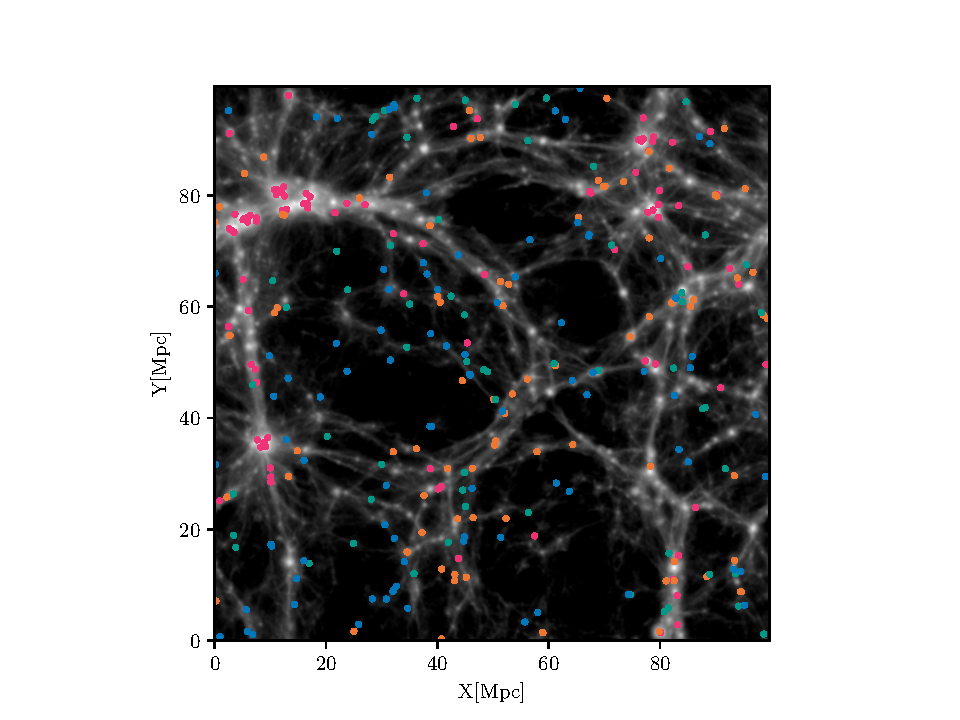
\includegraphics[width=2.\columnwidth]{plots_parent_sample/void_image_paper.pdf} 	
    \caption{ A slice of $100\times100\times 25\,\pMpc$  of galaxies in the simulation \REF~ at $z=0$. Each colour represent different galaxy sample with the same number density:  blue and green circles represent inner void and outer void galaxies whereas orange and magenta circles represent wall and skeleton galaxies.}   
     \label{fig:xydiagram}
\end{figure*}

We calculate  the distances between the centre of each galaxy, defined as the position of the minimum potential well, and  the centre of all voids (given  by the void catalogue). We associate each galaxy with the void whose centre is the closest to the galaxy. This ensures that  each galaxy  is associated with only one void.
To determine the environmental  effects of the large structure on the galaxies, we explore the shape of the void density profiles normalised by the mean density of the simulation as shown in  Fig.~7 of \citealt{paillas2017}. The density of the voids in the inner part is almost constant and much smaller than the mean density of simulation whereas in the external part of the void, the density increases mildly. At the boundary of the void, the density sharply increases and in the region outside of the void increases and decreases. At large radius, the density remains as the average in the simulation. Taking into account this, we split the selected galaxies into four samples depending on the relative location in terms of the radius of the closest void:
\begin{itemize}
    \item {\bf inner void} galaxies are defined as those whose centre is separated to the closest void  by a distance  between $0$ and $0.8\Rvoid$, where $\Rvoid$ is the radius of the closest void.
    \item {\bf outer void} galaxies whose separation to the closest void is   between $0.8\Rvoid$ and $\Rvoid$. 
    \item {\bf wall} galaxies are those located  between $\Rvoid$ and $1.4\Rvoid$. 
    \item {\bf skeleton} galaxies located beyond $1.4\,\Rvoid$. 
    
\end{itemize}
In total, we identified 513 inner void galaxies, 588 outer void galaxies, 3932 wall and  8167 skeleton galaxies of which  492, 528, 2574 and 3806  are centrals, respectively. Note that  each sample have a different fraction of satellites galaxies with the skeleton sample having a fraction of  $\sim 0.63$ of satellites  whereas $\sim 0.05$ of the void galaxies  are satellites. Then,  hereafter, we only focus on central galaxies in each sample. 


To visually inspect our classification, Fig.~\ref{fig:xydiagram} shows the dark matter density map of a slice of 100x100x25$\cMpc$ in the simulation \REF. Circles represent our selected galaxies and colours correspond to different samples. From the figure is clear that inner void galaxies (blue circles) are in the less dense regions of the simulations, as expected,  whereas skeleton galaxies (magenta circles) are found in the highest-density regions in the simulation. Outer Void (green circles) and wall galaxies (orange circles) are located in intermediate dense zones. 


\section{Results}
In this section, we describe  the properties of galaxies for the four parent galaxy samples as defined in section~\ref{subsection:galaxysample}, then we will compare sub-samples of each parent galaxy sample  with the same stellar mass distribution. Finally, we compare the sub-samples of each parent galaxy sample with similar  stellar mass and halo mass distribution. 

\subsection{Galaxy properties of inner void, outer void, wall and skeleton galaxies}

%In this subsection  we compare the galaxy properties for the four parent galaxy samples defined in section~\ref{subsection:galaxysample}. 
In the top  panel of  Fig.~\ref{fig:gmf} we show the stellar mass distribution of each parent galaxy sample. 
We find that the stellar mass distribution of inner void galaxies (blue solid lines) are systematically  biased to lower stellar mass, with a median stellar mass of $10^{9.4}\Msun$. This is lower than the median value obtained by using all galaxies in the simulation (grey lines) with a median of $10^{9.6}\Msun$, performing a KS test (p-value $\sim 10^{-9}$), we find that inner void galaxies has statistically  different stellar distribution from the total galaxy population. The median stellar mass systematically decreases from $10^{9.4}\Msun$ for inner void galaxies to  $10^{9.6}\Msun$  for  skeleton galaxies. With a KS test,  we find that galaxies in outer, wall and skeleton samples are not draw by the same population as inner void galaxies (with the highest  p-value $<0.08$ for outer void galaxies, and p-values $<1.e-9$ for  skeleton and wall galaxies). 



\begin{figure}	
	% To include a figure from a file named example.*
	% Allowable file formats are eps or ps if compiling using latex
	% or pdf, png, jpg if compiling using pdflatex
	\begin{tabular}{c}
	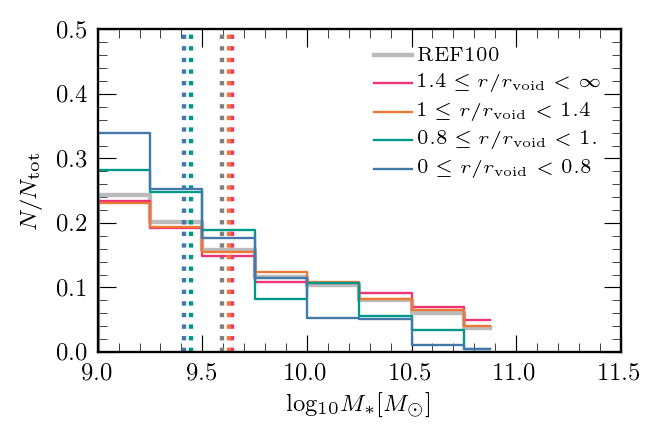
\includegraphics[width=1\columnwidth]{plots_parent_sample/GMF_cs_three_regions.png} \\
	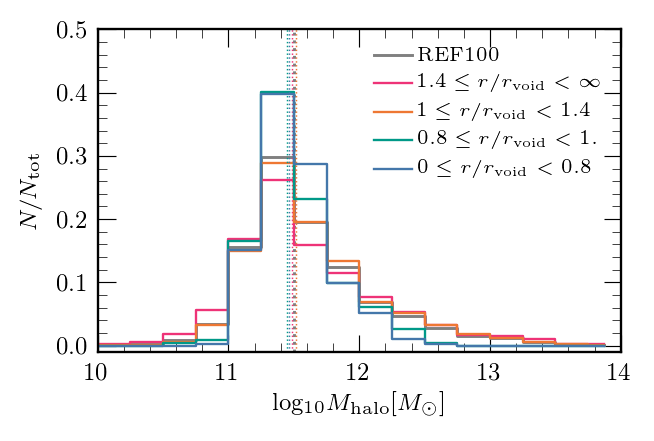
\includegraphics[width=1\columnwidth]{plots_parent_sample/HMF_cs_three_regions.png}\\
	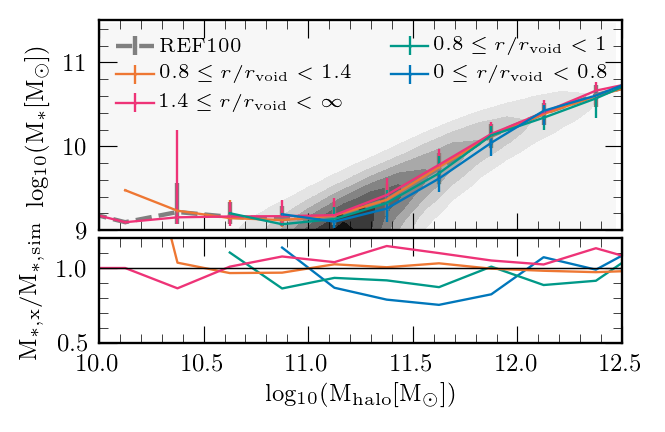
\includegraphics[width=0.95\columnwidth]{plots_parent_sample/Mstar_Mhalov2.png} 
	\end{tabular}	
    \caption{ Inner void, outer void, wall and skeleton galaxies are shown as blue, green, orange and magenta colours, respectively. Grey colour represents all the central galaxies in the simulation. \textit{Top panel:} The stellar mass distribution of each parent galaxy sample. Vertical dotted lines represent the median stellar mass for each parent galaxy sample. Inner void galaxies are biased towards galaxies with low stellar mass.  \textit{Middle panel:}The halo mass distribution. Vertical dotted lines represent the median halo mass.  \textit{Bottom panel:} The mean Halo mass-stellar mass relation for the four parent galaxy samples and the all centrals in the simulation.}
    %\textcolor{green}{Nelson: it would be nice to have a sub-panel with the ratio of the stellar mass to %halo mass for the different environments to see more clearly the differences here.}}
    \label{fig:gmf}
\end{figure}



%\textcolor{red}{Enrique: This points in the right direction, but it would be good to quote the errors (maybe standard error on the median). The difference is small and might be within the statistical fluctuation.}
%\textcolor{green}{Nelson: in Figure 1 the "wall" galaxies are referred to as "wall" galaxies, and I agree with Enrique that this is better! }

When the stellar mass distribution of inner void is compared to those of the outer void (green), wall (orange) and skeleton (magenta) regions, we find  that the fraction of massive galaxies ($\geq 10^{10}\Msun$) decreases systematically from the wall of the voids (orange colour) to the inner void regions (blue colour), so that above 12 per cent  of inner void galaxies  have  a stellar mass $\geq 10^{10}\Msun$). In contrast, 35 per cent of skeleton galaxies are as massive. These differences are consistent with those found by  \citet{ricciardelli2014} using cosmic voids identified in SDSS DR7. The authors compared void galaxies against wall galaxies and a control sample representing the total population of their sample, finding that low dense regions are biased towards low mass galaxies. 

The fact that the parent samples  have different stellar mass distributions is also reflected in the halo mass distribution, as shown in the middle  panel of Fig.~\ref{fig:gmf}. The halo mass distributions present a  peak distribution with a median halo mass slightly decreasing from $10^{11.50}\Msun$ in void wall  galaxies (orange)  to $10^{11.43}\Msun$ in inner void galaxies (blue). Note, however, that skeleton  galaxies (magenta) and void wall galaxies (orange) present a tail of massive halos ($M_{200}>10^{12}\Msun$) and a higher fraction of low mass halos ($<10^{12}\Msun$) in comparison with outer void (green) and inner void regions (blue).     

The bottom panel of Fig.~\ref{fig:gmf} present the halo mass-stellar mass relation for the four parent galaxy samples and summarises our results. The smallest haloes of the simulation are found in skeleton and void wall galaxies. Similarly, the most massive halos in the simulation  are only found in skeleton and void wall regions. It is interesting to mention that for a given halo mass between $10^{10.5}\Msun$ and $10^{12.5}\Msun$, the median stellar mass is systematically lower as a function of the location of the void. We find that for a given halo mass, the stellar mass is lower in galaxies located  in the inner void region (blue lines), and  is higher for those galaxies in the skeleton of the web. This is more clear in the last bottom panel that shows the  ratio between the median stellar mass in each subsample and the median stellar mass of the total central galaxy population for a given halo mass.   





\textcolor{green}{Nelson: can you show the average concentration or redshift of half mass in main branch of the haloes?  Iven if they are of similar mass, perhaps the different stellar masses in different environments are due to different secondary halo properties.}

Taking these  into consideration, it is expected to find some differences in the galaxy properties. Fig.~\ref{fig:fractionvoids} shows the fraction of star forming galaxies,  galaxies with atomic gas and  the fraction of disc galaxies as a function of void-centric distance . .. 
as a function of 

\begin{figure*}	
	% To include a figure from a file named example.*
	% Allowable file formats are eps or ps if compiling using latex
	% or pdf, png, jpg if compiling using pdflatex
	\begin{tabular}{cc}
	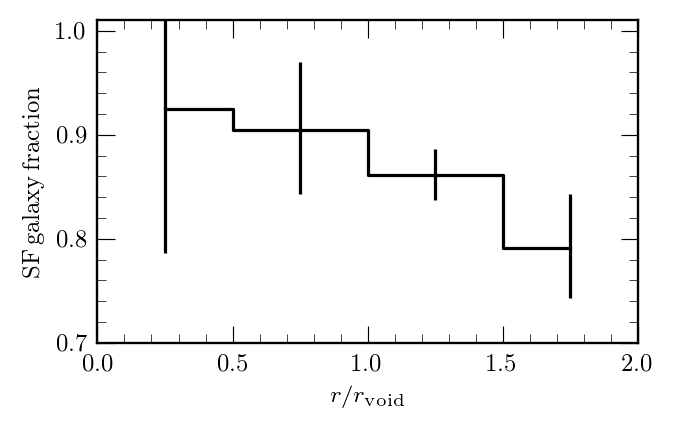
\includegraphics[width=\columnwidth]{plots_parent_sample/SFgal_fraction.png} &
	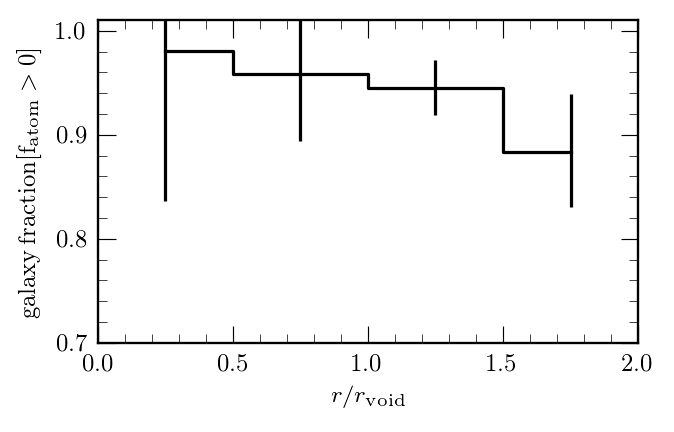
\includegraphics[width=\columnwidth]{plots_parent_sample/gasgal_fraction.png}\\
	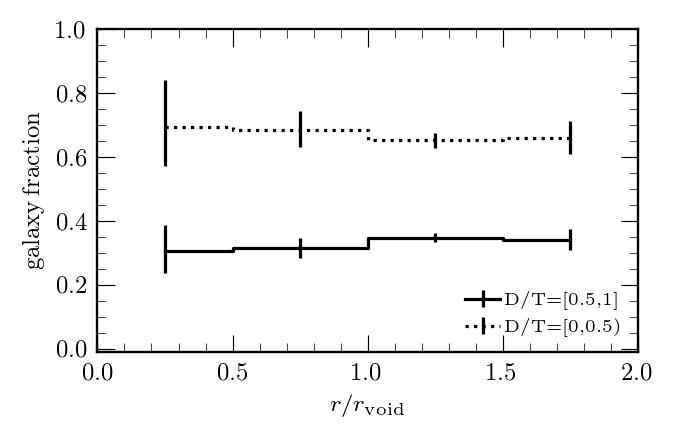
\includegraphics[width=\columnwidth]{plots_parent_sample/discgal_fraction.png} &
	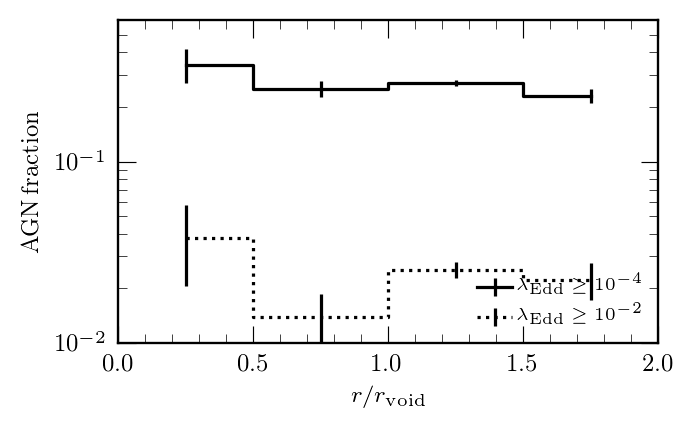
\includegraphics[width=\columnwidth]{plots_parent_sample/ActiveAGN_fraction.png} \\
	  
	\end{tabular}	
    \caption{ \textit{Top left panel:} Fraction of star forming galaxies as a function of the void-centric distance. Star  forming galaxies are considered with $\rm sSFR>10^{-11} Gyr^{-1}$. \textit{Top right panel}:Fraction of galaxies with $f_{\rm atom}>0$ as a function of the void-centric distance  where $f_{\rm atom}= 1.35 M_{\rm HI}/ (M_{*} +1.35 (M_{\rm HI} +M_{\rm HII}))$. \textit{Bottom left panel:} Fraction of disc ($D/T\geq 0.5$) and elliptical  galaxies ($D/T<0.5$) as a function of void-centric distance. \textit{Bottom right panel:}Active black holes as a function of the void-centric distance. Error bars in the plots correspond to Poisson errors. }
    \label{fig:fractionvoids}
\end{figure*}



\subsection{Sub-samples with equal stellar mass distribution}

\subsubsection{Galaxy Properties}
\begin{figure}	
	% To include a figure from a file named example.*
	% Allowable file formats are eps or ps if compiling using latex
	% or pdf, png, jpg if compiling using pdflatex
	\begin{tabular}{c}
	\includegraphics[width=1\columnwidth]{plots_stellarmass_central/GMF_cs_three_regions.png} \\
	\includegraphics[width=1\columnwidth]{plots_stellarmass_central/HMF_cs_three_regions.png}\\
	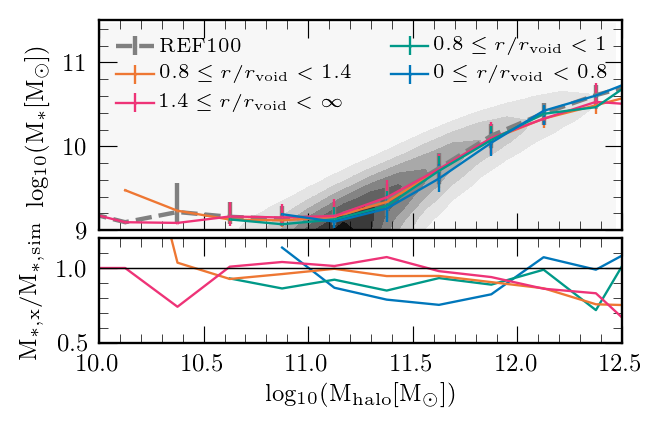
\includegraphics[width=0.95\columnwidth]{plots_stellarmass_central/Mstar_Mhalov2.png} \\
	\end{tabular}	
    \caption{ Sub-samples of the outer void (green colour), wall (orange colour) and skeleton (magenta colour) galaxies with a similar stellar mass distribution to the one of inner void galaxies. Grey colour represents all the central galaxies in the simulation. \textit{Top panel:} The stellar mass distribution of each galaxy sub-sample. Vertical dotted lines represent the median stellar mass for each galaxy sub-sample and compared to the parent sample of inner void galaxies. \textit{Middle panel:} The mean halo mass-stellar mass relation for the four galaxy sub-samples and all centrals in the simulation. \textit{Bottom panel:} The halo mass distribution. Vertical dotted lines represent the median halo mass.}
    \label{fig:gmf_samestellarmass}
\end{figure}

To determine how the results depend on galaxy stellar mass for the four parent samples, we select  
sub-samples of outer void, wall and skeleton galaxies such that they share the same stellar mass distribution  as  the inner void galaxies. The top panel of Fig.~\ref{fig:gmf_samestellarmass} shows the stellar mass distribution with vertical dotted lines the median stellar mass of each sample which remains almost constant for all the sub samples. For comparison, we included the stellar mass distribution of the total population as well as the median stellar mass. Note that the sub-samples are biased for the low mass galaxies  with a median stellar mass of $10^{9.41}\Msun$ whereas the median stellar mass with all central galaxies is $10^{9.6}\Msun$. 

%\textcolor{green}{Nelson: why not do this restriction of stellar mass distributions from the very beginning?  The conclusions do not change in any of the plots, perhaps the bimodality in the color goes away but it wasn't extremely clear before either.  If not, then select only a few of these figures (if at all) or simply mention results are stable under this selection.  I would prefer to see this selection from the beginning though.}

The bottom panels of Fig.~\ref{fig:gmf_samestellarmass} shows the halo mass distribution for the sub-samples  and the inner void galaxies. The sub-samples of skeleton and wall and outer void galaxies  present systematically higher fractions of lower mass halos than that from the inner void galaxies. Likewise the stellar mass distribution, the halo mass is biased lower massive haloes such that the most massive halos have a halo mass smaller than $10^{13}\Msun$. This is projected in the median halo mass of each sub-sample which falls systematically from the sub-sample of skeleton galaxies with a median $M_{200}=10^{10.32}\Msun$ to the parent sample of the void galaxies with  a median  $M_{200}=10^{10.43}\Msun$. Looking at the halo mass-stellar mass relation in the middle panel of Fig.~\ref{fig:gmf_samestellarmass}, we still find that for a given halo mass between $10^{11}\Msun$ and $10^{12}$, the stellar mass is lower in inner void galaxies than in skeleton galaxies. Additionally, there is a tail of low mass halos in the sub-samples of skeleton and wall galaxies, as well as, there is a small fraction of haloes with a mass larger than the maximum mass of the inner void galaxies. 


These differences in the halo mass distribution could be reflected in the galaxy properties.  
Fig.~\ref{fig:samestellarmass}  exhibit the same  galaxies properties from those shown in Fig.~\ref{fig:parentsamples} but for the sub-samples of  outer void, wall and skeleton galaxies. These sub-samples are compared with the parent galaxy sample of inner void galaxies. From the figure, it is clear that some of the differences seen in the galaxy properties of  the original samples are preserved.  For instance, the distribution of u-r (top left panel of Fig.~\ref{fig:samestellarmass}) retained the bimodal distribution  found in the parent samples of skeleton and wall galaxies with a small peak corresponding to the red, quenched massive galaxies  whereas there is an uni-modal distribution in inner void and outer void galaxies with a peak in the blue part of the distribution. Similar differences are found in the distribution of g-i (not shown here). Although, the median of u-r  of the sub-samples (see  vertical dotted lines) is just below to the one from the simulation (grey colour) that is 1.51 and similar to the median u-r from the inner void galaxies (1.49).    




\begin{figure*}	
	% To include a figure from a file named example.*
	% Allowable file formats are eps or ps if compiling using latex
	% or pdf, png, jpg if compiling using pdflatex
	\begin{tabular}{cc}
	%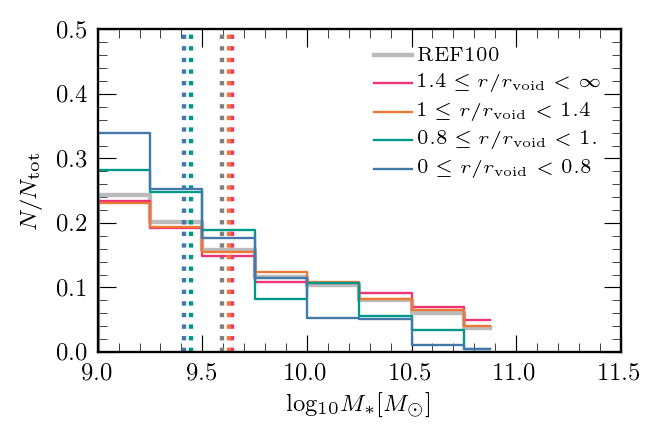
\includegraphics[width=1\columnwidth]{plots_parent_sample/GMF_cs_three_regions.png} &
	

	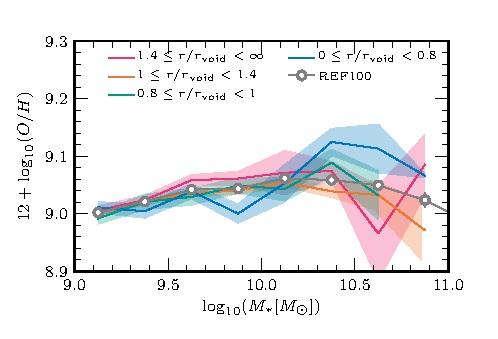
\includegraphics[width=1\columnwidth]{plots_stellarmass_central/mass_metallicity_threeregions_v1.pdf} &
	%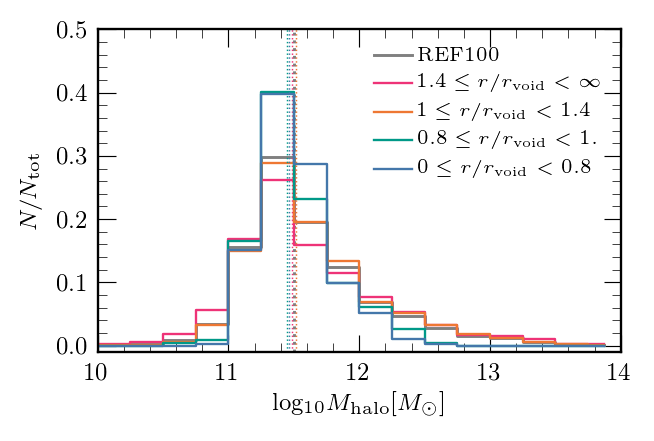
\includegraphics[width=0.95\columnwidth]{plots_parent_sample/HMF_cs_three_regions.png} &
 	\includegraphics[width=1\columnwidth]{plots_stellarmass_central/mass_ssfr_threeregions.pdf} \\
    
	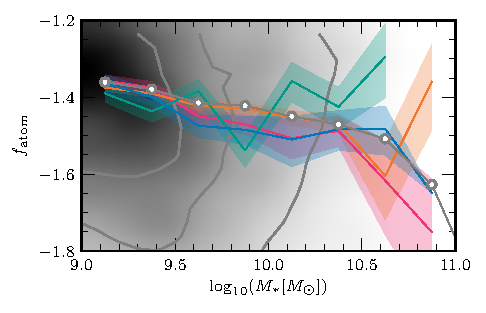
\includegraphics[width=1\columnwidth]{plots_stellarmass_central/mass_gasatomfrac_threeregions.pdf}  &
	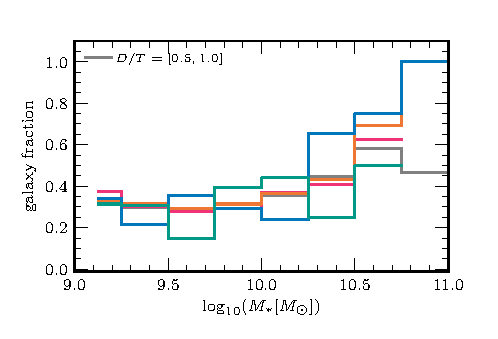
\includegraphics[width=1\columnwidth]{plots_stellarmass_central/mass_galfrac_morphology_threeregions_v1.pdf} \\
    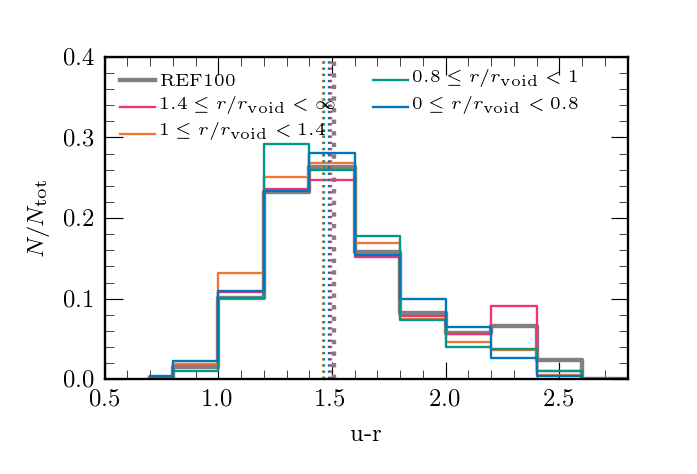
\includegraphics[width=1\columnwidth]{plots_stellarmass_central/u_r_fraction_threeregions.png}  &
	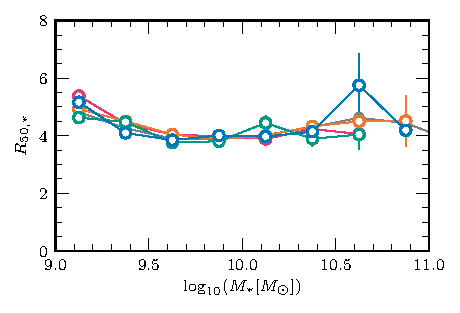
\includegraphics[width=1\columnwidth]{plots_stellarmass_central/mass_sizes_threeregions_PTcalsReff.pdf} \\	
	
	\end{tabular}	
    \caption{Galaxy properties of the galaxy sub-samples of outer void, wall and skeleton galaxies that are defined by the void centric distance as the legend indicates: outer void (green), wall (orange) and skeleton (magenta) galaxies. These sub-samples are selected such as they have the same stellar mass distribution as the parent sample of inner void galaxies. Grey colour represents all the central galaxies in the simulation. \textit{Top left panel:} Distribution of u-r for each sub sample and the galaxy parent sample of inner voids. \textit{ Top right panel:} The mean relation between stellar mass  and the star forming gas-phase  oxygen abundance.  Shaded regions represent the error of the mean of each sample and diffused markers correspond to galaxies in bins with less than 5 galaxies. \textit{ Bottom left panel:} The mean specific star formation rate (sSFR) as a function of the stellar mass. Coloured marker and solid lines represent the mean distribution and error bars represent the error of the mean. Diffused  stars correspond to galaxies in stellar mass bins with less than 5 galaxies. Grey contours and the diffuse density map represent all the central star forming  galaxies in the simulation. \textit{Bottom right panel:} The mean half-stellar mass radius as a function of the stellar mass for each parent galaxy sample. Shaded regions correspond to the error of the mean and grey markers for all the simulation. Diffused markers correspond to observation data from  Fernandez-Lorenzo et al.2013. }
    \label{fig:samestellarmass}
\end{figure*}


 %For instance, the  u-r histogram  for the different parent samples is shown in Fig~\ref{fig:parentsamples}. Clearly, skeleton galaxies present the typical bimodal distribution where the second peak corresponds to red and old, and usually massive, galaxies whereas inner void galaxies present an uni-modal distribution with a peak in the blue region. Note that outer void galaxies present a higher fraction of blue galaxies. On average, the outer void galaxies are bluer with a median u-r  of $1.46$ than inner void with $1.49$, following  wall galaxies with $1.50$ and skeleton galaxies with $1.54$. \textcolor{green}{Nelson: but stellar masses are different for each sample.  Is it possible to see median color vs. Mstellar? The bimodality in the red line is tenous at best in any case.}
%\begin{figure*}	
	% To include a figure from a file named example.*
	% Allowable file formats are eps or ps if compiling using latex
	% or pdf, png, jpg if compiling using pdflatex
	%\begin{tabular}{cc}
	%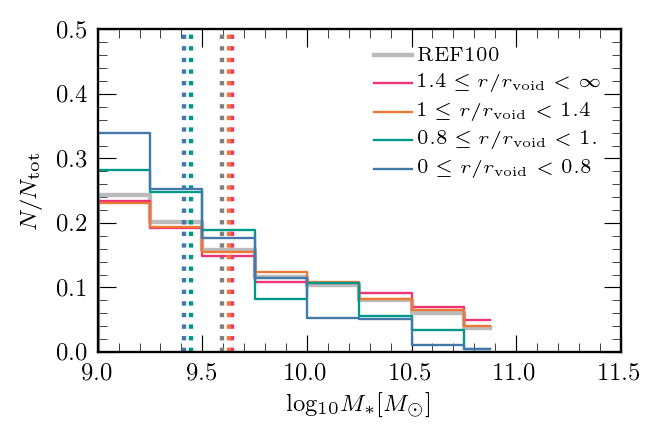
\includegraphics[width=1\columnwidth]{plots_parent_sample/GMF_cs_three_regions.png} &
	
	%\includegraphics[width=1\columnwidth]{plots_parent_sample/u_r_fraction_threeregions.png} & 
	%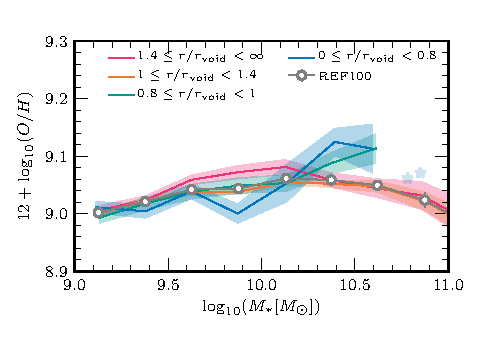
\includegraphics[width=1\columnwidth]{plots_parent_sample/mass_metallicity_threeregions_v1.pdf} \\
	%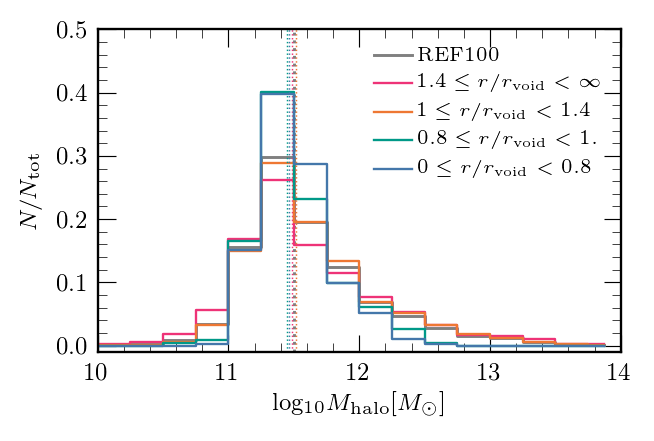
\includegraphics[width=0.95\columnwidth]{plots_parent_sample/HMF_cs_three_regions.png} &
 	%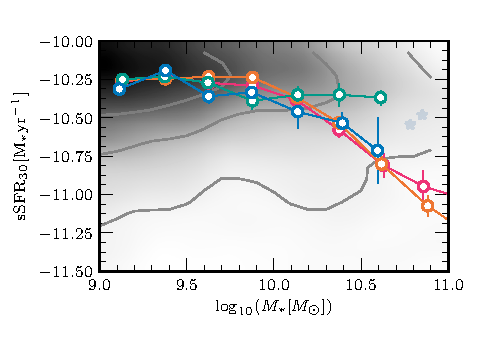
\includegraphics[width=1\columnwidth]{plots_parent_sample/mass_ssfr_threeregions.pdf} &

	%\includegraphics[width=1\columnwidth]{plots_parent_sample/mass_sizes_threeregions_stars.pdf} \\
	%\end{tabular}	
    %\caption{Galaxy properties of the four parent-galaxy samples selected as a function of the void centric-distance as indicated in the legend: inner void (blue), outer void (green), wall (orange) and skeleton (magenta) galaxies. Grey colour represents all the central galaxies in the simulation. \textit{Top left panel:} Distribution of u-r for each parent galaxy sample. \textit{ Top right panel:} The mean relation between stellar mass  and the star forming gas-phase  oxygen abundance for the four parent galaxy samples.  Shaded regions represent the error of the mean of each sample and diffused markers correspond to galaxies in bins with less than 5 galaxies. \textit{ Bottom left panel:} The mean specific star formation rate (sSFR) as a function of stellar mass. Coloured marker and solid lines represent the mean distribution and error bars represent the error of the mean. Diffused  stars correspond to galaxies in bins with less than 5 galaxies. Grey contours and the diffuse density map represent all the central star forming  galaxies in the simulation. \textit{Bottom right panel:} The half-stellar mass radius as a function of stellar mass for each parent galaxy sample. Error bars correspond to the error of the mean and grey markers for all the simulation.}
    %\label{fig:parentsamples}
%\end{figure*}
 
 
 
One of the most important properties that characterise  a galaxy is the rate at which is forming stars.  Bottom left panel of Fig.~\ref{fig:parentsamples} shows the specific star formation rate (sSFR)-stellar mass plane for the inner void, outer void, wall and skeleton  star forming galaxies where the sSFR is calculated in a 30-pkpc aperture. The solid lines with thicker markers represent the mean distribution and error bars the error of the mean of each sample. For stellar mass bins with less than 5 galaxies, the galaxies are presented as diffused stars instead.  Grey contours represent all the star forming galaxies in the simulation with a stellar mass larger than $10^9\Msun$ and sSFR$=10^{[-10,-11.5]}\rm yr^{-1}$. The figure shows that for the inner void, wall and skeleton regions most of the low stellar mass galaxies are active ($M_{*}\leq10^{10}\Msun$), near the region of the main sequence of the star forming galaxies, whereas massive galaxies are less active reaching values typical of quenched systems. In the case of the outer void region, massive galaxies are still active for the most massive stellar mass bin. This might be caused by the availability of gas supply to feed star formation since these regions have intermediate densities and hence the effects of the environment that can quench galaxies are expected to be less important. On the other hand galaxies in the voids might not be able to re-accrete enough gas to continue the star formation process.  Overall, we find that the star forming activity of the galaxies increases with the distance to the void-centre such that  inner and outer  void star forming galaxies present lower sSFRs,  with a mean of $10^{-10.31}\rm yr^{-1}$ and $10^{-10.28} \rm yr^{-1}$ respectively, than wall and skeleton star forming galaxies with a mean sSFR of   $10^{-10.37} \rm yr^{-1}$ and $10^{-10.40} \rm yr^{-1}$. 


Another important property that characterises a galaxy is the average metallicity since encapsulates the assembly history of a galaxy.  In particular, it  constrains how the gas has been reprocessed by stars and by different types of exchanges with their surroundings. The top right panel of Fig.~\ref{fig:parentsamples} shows the mean relation between the star forming gas phase oxygen abundance and the stellar mass for the star forming galaxies in each parent sample. We also include all central galaxies (grey colour) in the simulation for comparison. Clearly, the oxygen abundances of inner and outer void star forming  galaxies (blue and green respectively) increase by more than $\sim 0.1$ dex with stellar mass and flatten in massive star forming galaxies ($M_{*}\gsim10^{10.4}\Msun$). In contrast, the mean oxygen abundances of  wall (orange) and skeleton (magenta) star forming galaxies mildly increase at low stellar mass and decrease again for massive galaxies($M_{*}\gsim10^{10.4}\Msun$).     This behaviour is similar to the mean relation of all galaxies in the simulation (grey colour and circles).  

When we compare each parent sample at low stellar masses, inner void star forming galaxies present  the lowest oxygen abundances  whereas  skeleton star forming galaxies present the highest values of oxygen abundances. The behaviour is the opposite for inner void massive galaxies that  present higher oxygen abundances in comparison with those from wall and skeleton massive  galaxies. Despite the differences found at a given stellar mass, overall, the mean oxygen abundances of the star-forming gas phase remain roughly constant as a function of  their location to the void centre where the mean oxygen abundances are 9.02, 9.03, 9.03 and 9.04  for  inner void, outer void, wall and skeleton galaxies respectively. \textcolor{red}{Enrique: What could be a possible explanation for this inversion (higher oxygen abundance for massive inner galaxies, but }




%\begin{figure*}	
	% To include a figure from a file named example.*
	% Allowable file formats are eps or ps if compiling using latex
	% or pdf, png, jpg if compiling using pdflatex
%	\begin{tabular}{cc}
	%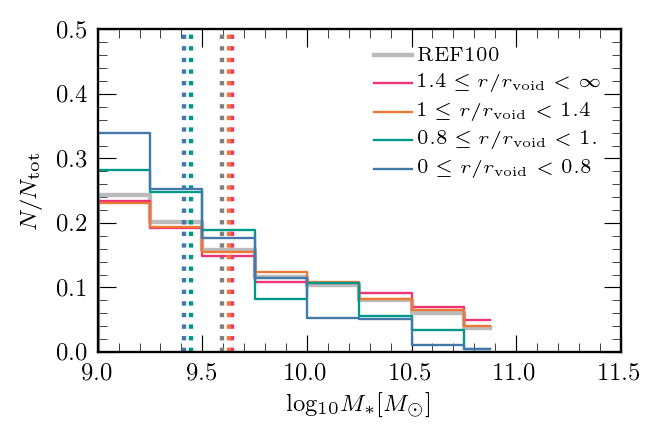
\includegraphics[width=1\columnwidth]{plots_parent_sample/GMF_cs_three_regions.png} &
	

	%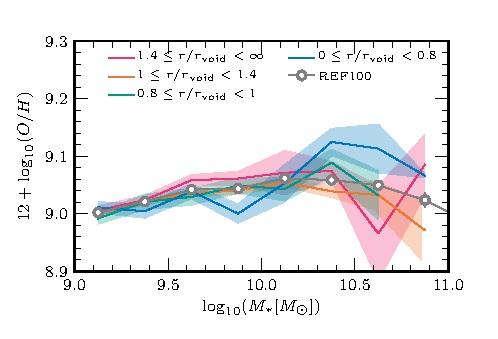
\includegraphics[width=1\columnwidth]{plots_stellarmass_central/mass_metallicity_threeregions_v1.pdf} &
	%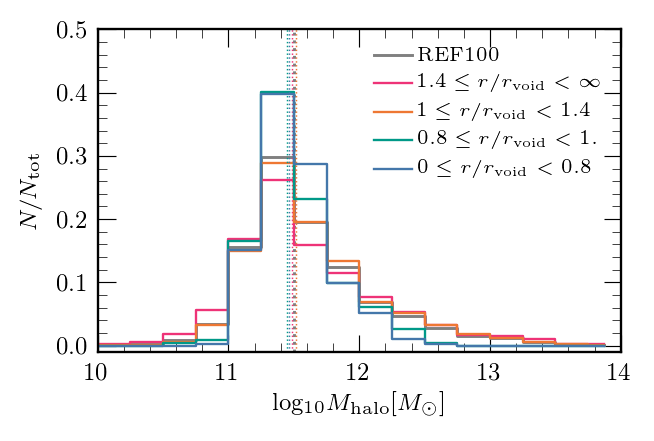
\includegraphics[width=0.95\columnwidth]{plots_parent_sample/HMF_cs_three_regions.png} &
 	%\includegraphics[width=1\columnwidth]{plots_stellarmass_central/mass_ssfr_threeregions.pdf} \\
%    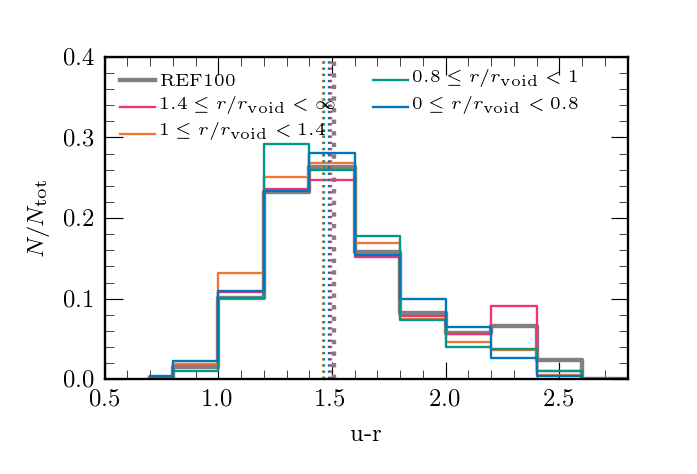
\includegraphics[width=1\columnwidth]{plots_stellarmass_central/u_r_fraction_threeregions.png}  &


%	\includegraphics[width=1\columnwidth]{plots_stellarmass_central/} \\
%	\end{tabular}	
%    \caption{Galaxy properties of the galaxy sub-samples of outer void, wall and skeleton galaxies that are defined by the void centric distance as the legend indicates: outer void (green), wall (orange) and skeleton (magenta) galaxies. These sub-samples are selected such as they have the same stellar mass distribution as the parent sample of inner void galaxies. Grey colour represents all the central galaxies in the simulation. \textit{Top left panel:} Distribution of u-r for each sub sample and the galaxy parent sample of inner voids. \textit{ Top right panel:} The mean relation between stellar mass  and the star forming gas-phase  oxygen abundance.  Shaded regions represent the error of the mean of each sample and diffused markers correspond to galaxies in bins with less than 5 galaxies. \textit{ Bottom left panel:} The mean specific star formation rate (sSFR) as a function of the stellar mass. Coloured marker and solid lines represent the mean distribution and error bars represent the error of the mean. Diffused  stars correspond to galaxies in stellar mass bins with less than 5 galaxies. Grey contours and the diffuse density map represent all the central star forming  galaxies in the simulation. \textit{Bottom right panel:} The mean half-stellar mass radius as a function of the stellar mass for each parent galaxy sample. Shaded regions correspond to the error of the mean and grey markers for all the simulation. Diffused markers correspond to observation data from  Fernandez-Lorenzo et al.2013. }
 %   \label{fig:samestellarmassv2}
%\end{figure*}




Finally, we look at the galaxy size that is another main characteristic of galaxies. The relation between stellar mass and galaxy size was established by  \cite*{shen2003} studying SDSS galaxies and without any selection by environment, finding that a strong correlation between stellar mass and galaxy size, especially for early-type galaxies.  
We present galaxy sizes as a function of stellar mass in the right panel of Fig.~\ref{fig:parentsamples}  for the four parent samples. We have also included as grey markers with solid lines the relation using the total central galaxy population.  We find that the galaxy size (defined as the radius that encloses 50 per cent of the stellar mass, $R_{50,*}$) increases with stellar mass for all the four parent galaxy samples and using all the central galaxies in the simulation. We do not find significant differences between the parent galaxy samples, except for  inner void massive galaxies  (blue solid line,$M_{*}\geq10^{10.4}\Msun$)  where galaxy sizes are higher than those from  outer void, wall and skeleton galaxies. \textcolor{green}{Nelson: I kind of see smaller sizes for void galaxies below logMstar10.5} This result is compared with observations (grey markers) from \cite*{fernandez-lorenzo2013} who studied the relation between the stellar mass and galaxy size of the most isolated galaxies in the local Universe.  The authors use data from the AMIGA project, defining the environment with two parameters: $Q$, the tidal strength created by all neighbours  and $\eta_{k}$ the local number density. They find that sizes of low mass galaxies in different environments are similar, especially for early-type galaxies, although for spiral massive galaxies the authors find  that the more isolated massive spirals are, larger their sizes. This is roughly in agreement with our findings, however, the galaxy size in AMIGA seem to be smaller than those from  EAGLE. 
Galaxy sizes from AMIGA also present some discrepancies  with those estimated from \cite*{shen2003} as in  \cite*{fernandez-lorenzo2013} is  pointed out, possibly caused  by the method used to estimate the half-mass radius. Since the EAGLE simulation was calibrated to reproduce the observed median galaxy size-stellar mass relation (and other properties) from  \cite{shen2003} with SDSS galaxies   and  \cite{baldry2012} with GAMA galaxies (see \citealt{schaye2015} for the details), it is expected to have these discrepancies between AMIGA and EAGLE. \textcolor{green}{Nelson: if the sizes have already been compared to observations by the EAGLE collaboration, better not to put observations here.}

 \subsubsection{BH properties in voids }
 
  \begin{figure*}	
	% To include a figure from a file named example.*
	% Allowable file formats are eps or ps if compiling using latex
	% or pdf, png, jpg if compiling using pdflatex
	\begin{tabular}{cc}
	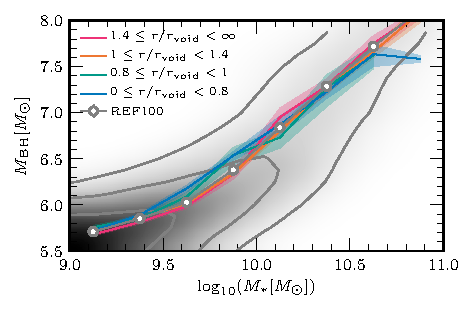
\includegraphics[width=1\columnwidth]{plots_stellarmass_central/mass_mbh_threeregions_v2.pdf} &
	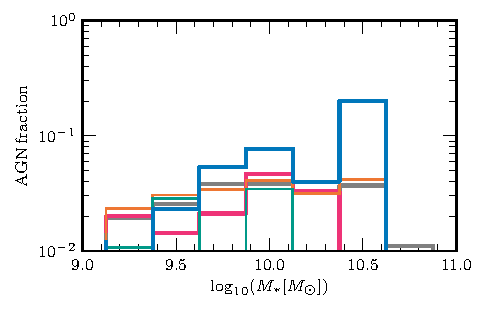
\includegraphics[width=1\columnwidth]{plots_stellarmass_central/mass_AGNfraction_threeregions_v1.pdf}\\
	
    \caption{BHs }
    \label{fig:BHs}
\end{figure*} 

 \subsubsection{Merger histories}
 \label{subsubsec:MHs}
 %\begin{figure*}	
	% To include a figure from a file named example.*
	% Allowable file formats are eps or ps if compiling using latex
	% or pdf, png, jpg if compiling using pdflatex
	%\begin{tabular}{cc}
%	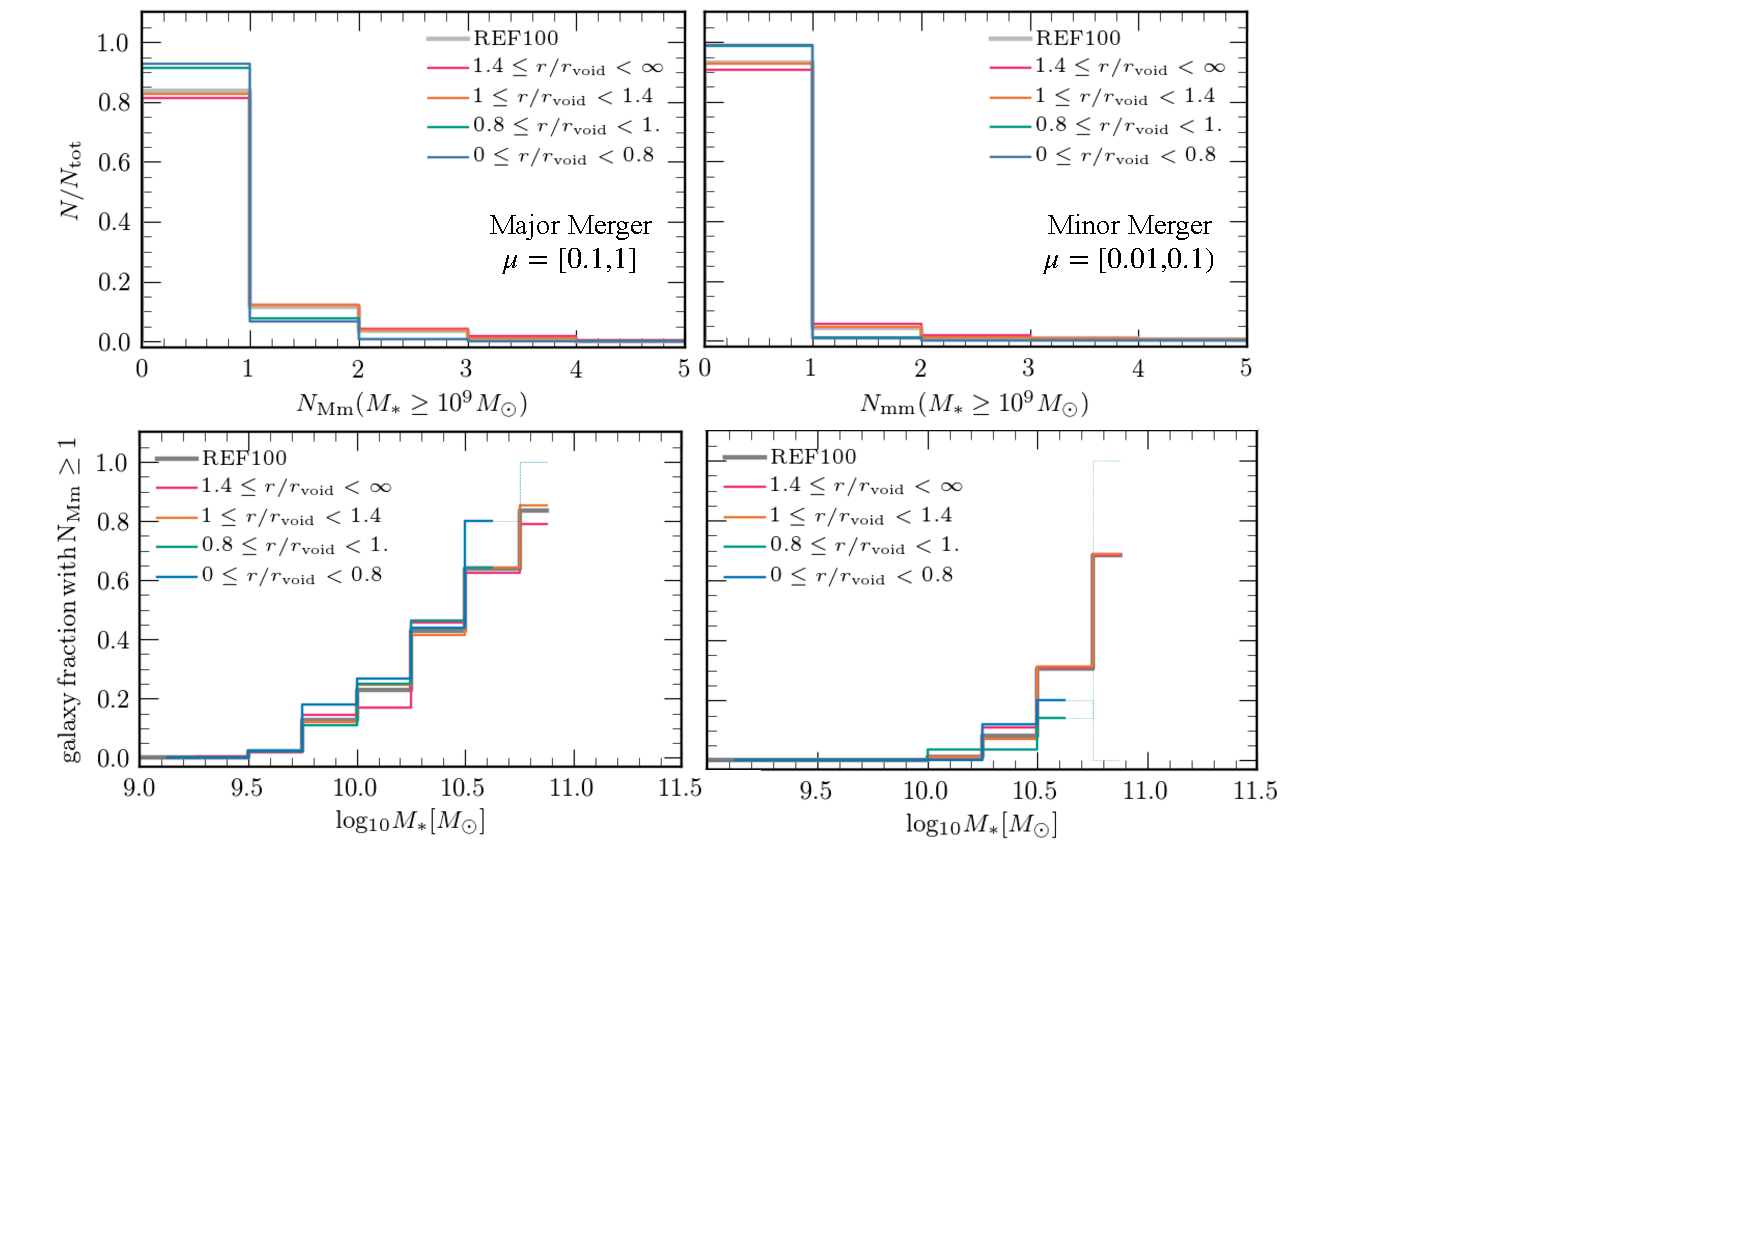
\includegraphics[width=2\columnwidth]{plots_parent_sample/Mergerplot_parentsample.pdf}  
%    \caption{Merger histories of the parent samples. Blue and green colours represent inner and outer void galaxies and orange and magenta colours represent wall and skeleton galaxies respectively. Grey lines represents all the central galaxies in the simulation. \textit{Top panels from left to right:} The distribution of the number of major/ minor mergers that galaxies experienced \textit{Bottom panel from left to right :} The fraction of galaxies that experienced at least a major/minor merger as a function of stellar mass. Thin dotted lines indicates stellar mass bins that contain less than 5 galaxies.}
 %   \label{fig:mergers}
%\end{figure*} 
 
 
 %\begin{figure*}	
	% To include a figure from a file named example.*
	% Allowable file formats are eps or ps if compiling using latex
	% or pdf, png, jpg if compiling using pdflatex
	%\begin{tabular}{cc}
	%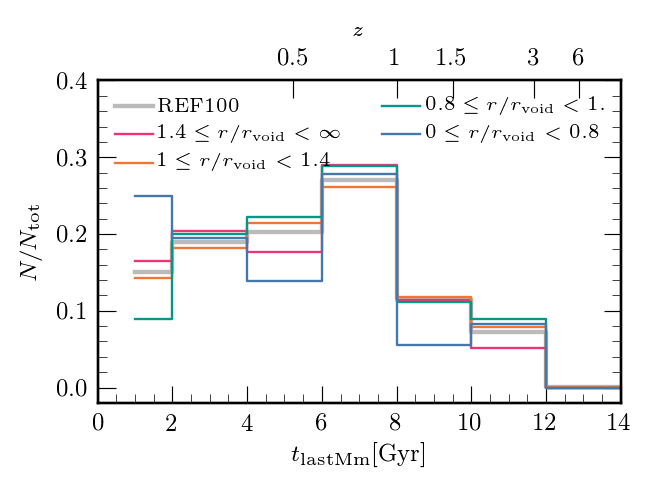
\includegraphics[width=1\columnwidth]{plots_parent_sample/distributionlastmajormerger_three_regions.png}  & 
	%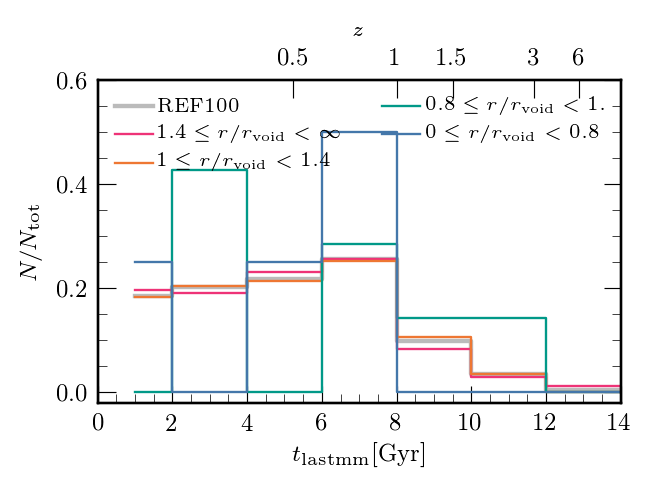
\includegraphics[width=1\columnwidth]{plots_parent_sample/distributionlastminormerger_three_regions.png} \\
	%\end{tabular}	
    %\caption{\textit{ From left to right:} Time distribution of the last major/minor merger a galaxy have experienced. Blue, green, orange and magenta lines correspond to inner void, outer void, wall and skeleton galaxies respectively. Grey lines represent all the galaxies in the simulation. \textcolor{green}{Nelson: make less bins for inner void, or even better, use cummulative distributions as in figure 10.}}
    %\label{fig:lastmergers}
%\end{figure*} 
 To further explore the differences in the parent samples defined by the distance to the closest void centre, we trace the merger histories of each galaxy. We count for the minor and major mergers that galaxies have experienced through cosmic time. We consider as major mergers when  the stellar mass ratio between the secondary galaxy and the primary galaxy, $\mu$ is higher than $0.1$, while minor mergers are defined for $\mu$  between $0.01$ and $1$. Stellar masses of the merging
galaxies are considered at the snapshot prior SUBFIND considered them as one structure. To ensure that galaxies have been properly followed, we only consider mergers with galaxies with stellar masses larger than $10^9 \Msun$. 

Top panels of Fig.~\ref{fig:mergers} from right to left  present the distribution of the number of  major and minor mergers that experienced inner void (blue), outer void (green), wall (orange) and skeleton (magenta) galaxies across cosmic time. As we expect inner void and outer void galaxies, which live in under-dense regions, have quiet  major and minor merger histories than wall and skeleton galaxies. The fraction of inner and outer  void galaxies that experienced at least one major (minor) merger are respectively  0.07 (0.01) and 0.08 (0.01),  whereas it  is   0.17 (0.07) and 0.19 (0.09) for wall and skeleton galaxies separately. 
Also, when inner void galaxies are compared to the total central galaxy population (grey lines), the galaxy fraction with at least one major (minor) merger is less than  a half (one seventh) of the galaxy fraction taking into account all the central galaxy population\textcolor{green}{Nelson: less mergers goes well with smaller size!}

The fraction of galaxies that suffered one major and minor  merger as a function of the stellar mass is shown  in the bottom panels of Fig~\ref{fig:mergers} from left to right. From the figure is clear that  the fraction of galaxies that underwent at least one major merger increases with mass for all the parent samples. Note, however, that more than 80 per cent of the most massive galaxies ($M_{*}\geq10^{10.5}\Msun$) in the inner region of voids experienced one major merger whereas  the most massive galaxies in outer void,  wall, skeleton galaxies present a percentage between  below 80.  Regarding minor mergers, only galaxies with a stellar mass larger than $10^{10}\Msun$ have experienced minor mergers for the four parent samples, possibly because of the resolution of the simulation and the stellar mass cut that we imposed in the merger histories. Inner void galaxies present a small percentage of galaxies that experienced a minor merger as a function of the stellar mass, reaching the maximum fraction at 20 for galaxies with a stellar mass of $10^{10.5,10.75}\Msun$ whereas the percentage of  wall and skeleton galaxies that experienced at least one minor merger increases with stellar mass  and are higher than the inner void galaxies reaching $\sim 70$ for the most massive galaxies. Note that inner and outer void galaxies count with less than 5 galaxies in the most massive bin (thin dotted lines), however, it is interesting that all the massive outer void galaxies ( $M_{*}\geq10^{10.75}\Msun$) underwent at least one minor merger.  
  
 
 Fig~\ref{fig:lastmergers} shows the time distribution when the last major (left panel) and minor merger (right panel) took place for those galaxies that experienced at least one major/ minor merger. As we can see in the right panel of the figure, the shape of the time distribution of the last major merger presents a peak $z\sim 0.6$ ($\sim 6$ Gyrs ago) for all the parent samples. However, the fraction of galaxies that experienced their last major merger above $z>0.6$ falls from  50 per cent in skeleton galaxies to 40 per cent for inner void galaxies. Moreover, there is about 25 per cent of the inner void galaxies that the last merger took place in the last 2 Gyrs whereas, for the wall, skeleton and  outer void galaxies, the percentage is lower than 18.     Similarly, the time distribution of the last  minor merger that took place peaks at $z\sim 0.6$, although  the galaxy fraction that suffered at least one minor merger is never above 0.3, except for the inner void galaxies  that peaks at  0.5. Note also that there is a galaxy fraction of 0.4 in the outer void regions that experienced their last minor merger between 2 and 4 Gyrs ago. 
 
 Overall, we find that inner void and outer void galaxies present quiet merger histories in comparison with wall and skeleton galaxies and also with the total  central galaxy population in the simulation. For inner and outer void galaxies that experienced at least one major/minor mergers, a quarter of them their last merger occurred in the last two Gyrs. This fraction is higher in comparison with  the fraction (less than  a fifth) of  wall and skeleton galaxies that experienced the last major/minor mergers in the last two Gyrs.  These differences could be thought as indicative of the effects of the (large-scale) environment. However, the halo mass and in the stellar mass distribution is different for the four galaxy samples. In the next sections,  we separate the effects of the stellar mass and the halo mass. 
 
 



The top left panel of Fig.~\ref{fig:samestellarmass} shows, instead, the sSFR-stellar mass plane for the sub-samples of outer void, wall and skeleton star forming  galaxies and are compared to the parent sample of inner void star forming  galaxies. Unlike the parent galaxy samples, we do not find significant differences in the star formation activity as a function of the distance of the void-centre. Although, the mean sSFR  of the sub-samples of wall and outer void galaxies ($10^{-10.28}\rm yr^{-1}$) tend to be lower than the one from the sub-sample of skeleton and inner void galaxies ($10^{-10.30}\rm yr^{-1}$). We also find that the star formation activity of the sub-samples is higher than the average from the original parent samples. This increment in the star formation activity  could be caused by the fact that galaxies residing in massive halos ($M_{200}>=10^{12.5}\Msun$) are likely to be red and quenched but they  are not included in the sub-samples of the skeleton, wall and outer void galaxies. Also, it is interesting that the star formation activity  in massive outer void galaxies ($M_{*}\geq10^{10}\Msun$) from the sub-sample is still higher in comparison with the sub-samples of  wall and skeleton galaxies and the parent galaxy sample of the inner void region. 

Regarding the relation of the star forming gas phase oxygen abundances  and stellar mass, the top right panel of Fig.~\ref{fig:samestellarmass} show the mean relation between gas phase oxygen abundance and stellar mass for each sub-samples. We also include  all the central galaxies in the simulation. From the figure, we see that inner void galaxies with a low stellar mass ($M_{*}<10^{10}\Msun$), still present slightly lower star-forming gas phase oxygen abundances in comparison with those from the sub-sample of skeleton galaxies. At higher mass, in contrast, the gas-phase oxygen abundances of the inner void significantly increase with time whereas those in skeleton and wall  galaxies in the sub-samples flatten with stellar mass. This might be also pointed out as an effect of the environment on the global gas-phase metallicity.     

We also explore the stellar mass-galaxy size relation. As in the parent samples, for galaxies with low mass ($M_{*}\leq 10^{10}\Msun$) we did not find  significant differences as a function of the void-centric distance. In the case  of massive galaxies, the differences are not clear since we have a low statistics of massive galaxies, although we can see a tendency of inner void and outer void galaxies to have larger sizes than their counterparts in walls and the skeleton of the web. 

\subsubsection{Merger histories}
\begin{figure*}	
	% To include a figure from a file named example.*
	% Allowable file formats are eps or ps if compiling using latex
	% or pdf, png, jpg if compiling using pdflatex
	%\begin{tabular}{cc}
	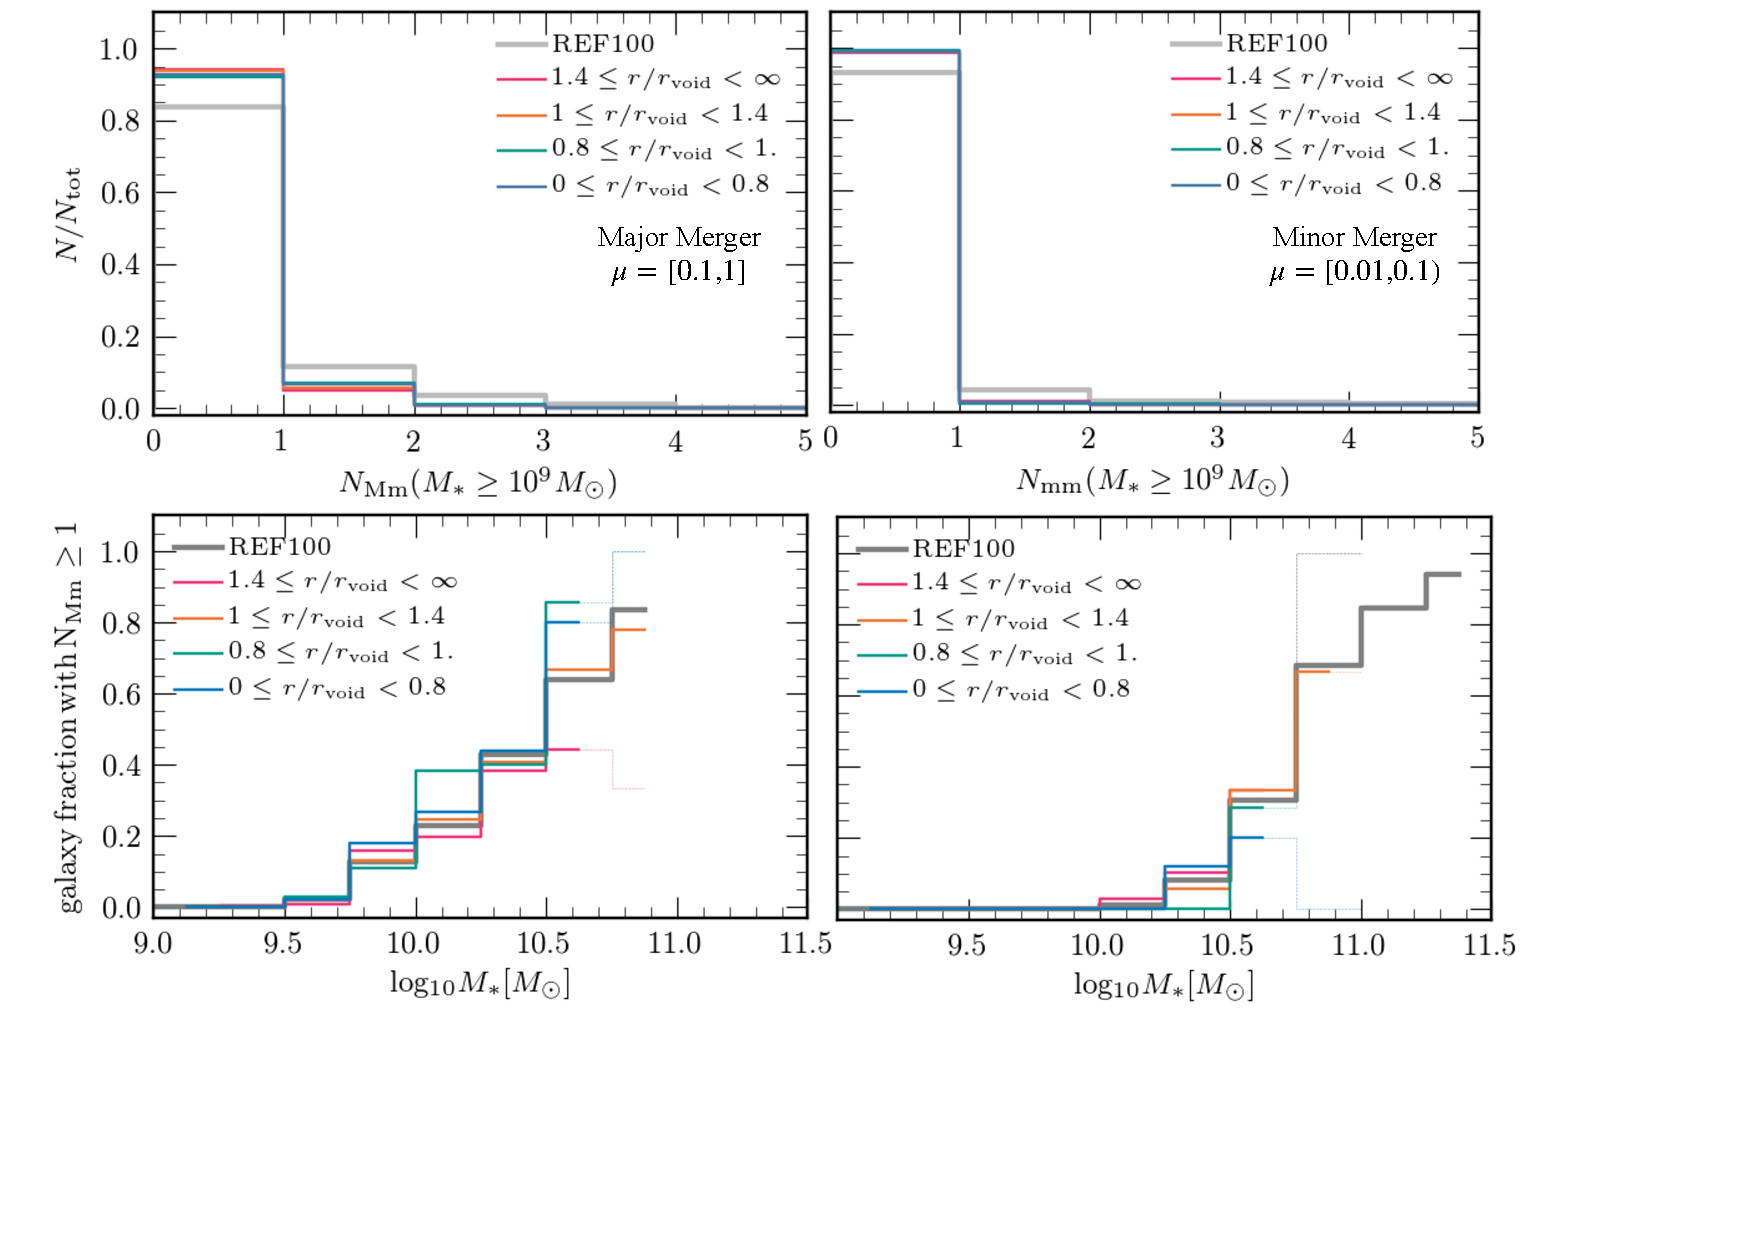
\includegraphics[width=2\columnwidth]{plots_stellarmass_central/merger_plot_ssm.pdf}  
    \caption{Merger histories of the sub-samples with similar stellar mass distribution as inner void galaxies (blue colour). Green, orange and magenta colours represent  outer void, wall and skeleton galaxies respectively. Grey lines represent all the central galaxies in the simulation. \textit{Top panels from left to right:} The distribution of the number of major/ minor mergers that galaxies experienced \textit{Bottom panel from left to right :} The fraction of galaxies that experienced at least a major/minor merger as a function of the stellar mass. Thin dotted lines indicates stellar mass bins that contain less than 5 galaxies.}
    \label{fig:mergers_ssm}
\end{figure*} 
 
 
 \begin{figure*}	
	% To include a figure from a file named example.*
	% Allowable file formats are eps or ps if compiling using latex
	% or pdf, png, jpg if compiling using pdflatex
	\begin{tabular}{cc}
	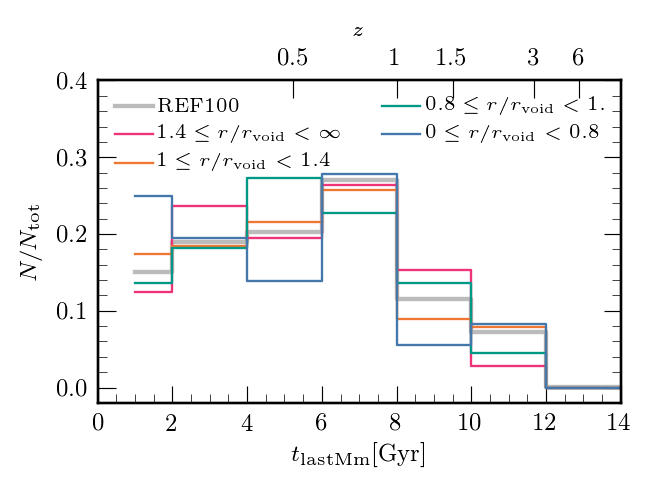
\includegraphics[width=1\columnwidth]{plots_stellarmass_central/distributionlastmajormerger_three_regions.png}  & 
	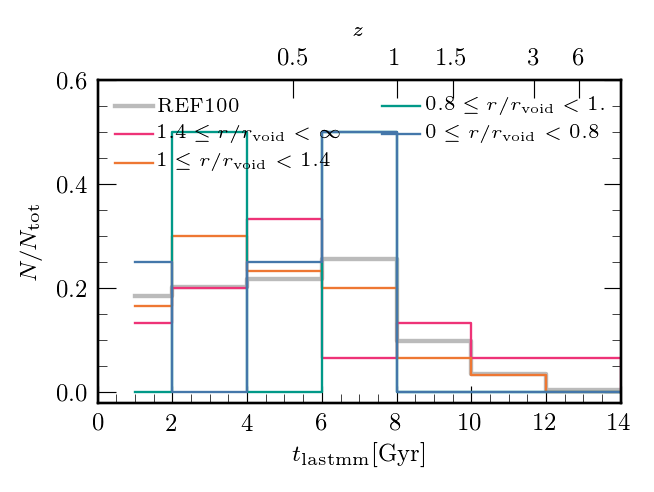
\includegraphics[width=1\columnwidth]{plots_stellarmass_central/distributionlastminormerger_three_regions.png} \\
	\end{tabular}	
    \caption{\textit{ From left to right:} Time distribution of the last major/minor merger a galaxy have experienced. Blue, green, orange and magenta lines correspond to inner void galaxies, the sub-samples of  outer void, wall and skeleton galaxies respectively. Grey lines represent all the galaxies in the simulation.}
    \label{fig:lastmergers_ssm}
\end{figure*} 


In this section, we explore the merger histories of the sub-samples of the outer, wall and skeleton galaxies and we  compare them to inner void galaxies.
 We use the definition of a major and minor merger as described in section~\ref{subsubsec:MHs}. 
Top panels of Fig.~\ref{fig:mergers_ssm} present number distribution of major (left panel ) and minor (right panel) mergers that galaxies underwent for inner void galaxies and for the sub-samples of outer void, wall and skeleton galaxies across time. Unlike the parent-galaxy samples, we find that there is no important discrepancy in the major (minor) merger histories as a function of void centric distance  for the sub-samples with same stellar mass distribution as inner void galaxies. These results could be because we ignore the most massive halos in the outer void, wall and skeleton galaxies  in order to match the stellar mass distribution of void galaxies. Also, the major and minor histories are quiet in comparison with those from all the central galaxy population (grey colour).  Similar to the parent samples, we find that the galaxy fraction that underwent at least one major/minor merger increases with stellar mass as shown in  bottom panels  of Fig.~\ref{fig:mergers_ssm}. In the case of major mergers,  massive inner void galaxies still exhibit a higher galaxy fraction  that underwent a major merger (80 per cent) in comparison with those from the sub-samples of skeleton and wall galaxies (below 60  per cent). In contrast, the sub-sample of massive wall galaxies exhibits the highest fraction of galaxies that experience at least one minor merger  whereas inner void galaxies present the lowest one. Note, however, that for massive galaxies, we account for a low statistics (less than 5 galaxies per stellar mass bin; thinner lines in the Figure) to notice  significant differences between the sub-samples of outer void,  and inner void galaxies. 

Fig.~\ref{fig:lastmergers_ssm} presents the time distribution of the last major (right panel) and minor (left panel) merger that took place for galaxies that suffered at least one major (minor) merger. The percentage of galaxies that underwent the last major merger at $z>0.6$( above 6 Gyrs ago ) is $\sim 40$ for all the sub-samples and inner void galaxies, with no significant difference between them. Also, the sub-samples of outer void ($\sim 14$ per cent), wall ($\sim 18$ per cent) and skeleton galaxies ($\sim 12$ per cent) present lower fractions of galaxies that suffered the last major merger 2 Gyrs ago than the fraction of inner void galaxies ($\sim 26$ per cent). Regarding the last minor merger, the time distribution of the last minor merger is shown in the right panel of Fig.~\ref{fig:lastmergers_ssm}.  Unlike the parent samples, the time distribution of the last minor merger occurred peaks at lower redshift for the sub-samples of  outer void galaxies and wall galaxies ($z\sim 0.3$) and skeleton galaxies ($z\sim0.5$) whereas the peak of the time distribution of last minor merger in inner void galaxies is at $z\sim 0.6$.   

In general, we find that the major (minor) merger histories from the sub-samples of outer void, wall and skeleton (with the same stellar mass distribution) are as quiet as those from inner void galaxies. Nonetheless, for the inner void galaxies that underwent at least one major/minor mergers  a quarter of them, the last major merger occurred in the last 2 Gyr ago whereas only a tenth of galaxies in  the sub-samples of outer void, skeleton, wall regions the last major merger happens during this time. For minor mergers, the peak of time distribution of the last merger occurred shifts at lower redshifts ($z\lsim 0.5$) for the sub-samples outer void, wall and skeleton galaxies whereas  the peak for inner void galaxies happens at $z\sim 0.6$.   


%\subsection{Galaxy properties for sub-samples with the same stellar mass and halo mass distributions}

%\begin{figure}	
	% To include a figure from a file named example.*
	% Allowable file formats are eps or ps if compiling using latex
	% or pdf, png, jpg if compiling using pdflatex
	%\begin{tabular}{c}
	%\includegraphics[width=1\columnwidth]{plots_halo_starmass_centrals/GMF_cs_three_regions.png} \\
	%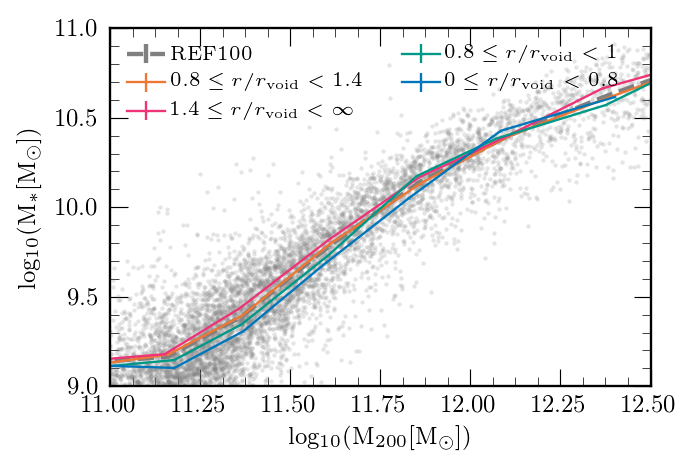
\includegraphics[width=0.95\columnwidth]{plots_halo_starmass_centrals/Mstar_Mhalo.png} 
	%  \\
	%\includegraphics[width=1\columnwidth]{plots_halo_starmass_centrals/HMF_cs_three_regions.png}\\
	%\end{tabular}	
    %\caption{The halos mass-stellar mass relation for  sub-samples of  outer void (green colour), wall (orange colour) and skeleton (magenta colour) galaxies with similar stellar mass and halo mass distributions as the parent galaxy sample of inner void galaxies.  Grey colour represent all the central galaxies in the simulation.}
    %\label{fig:gmf_shmsm}
%\end{figure}

%In the previous section, we find that galaxy sub-samples of outer void, wall and skeleton galaxies with similar stellar mass distribution as the one from inner void galaxies, present similar quiet merger histories and not significant differences, especially for low mass galaxies ($M_{*}\leq 10^{10}\Msun$) apart from the mean gas-phase abundances-stellar mass relation. For massive galaxies, even though we find differences in galaxy properties, we have a low number of  massive galaxies in each sub-sample to asses the significance of these differences.   
%In this section, we separate the possible effects of the halo mass on the galaxies properties. For that,  we select the sub-samples of outer void, skeleton and wall galaxies such that they have the same stellar mass distribution and halo mass distribution as those distributions in inner void galaxies. We also focus only on the galaxies between $M_{*}=10^{9}\Msun$ and $10^{11}$ and halos mass between $M_{200}=10^{11}\Msun$  and $10^{12}\Msun$ where we have sufficient data to draw some differences due to large scale environment.  Fig.~\ref{fig:gmf_shmsm} show the median halo mass-stellar mass relation for the sub-samples of skeleton, wall and outer void galaxies and compared with inner void galaxies. As in the figure is shown, the median halo mass-stellar mass relation  fluctuates by less than 0.01 dex in stellar mass for a given halo mass from the sub-samples of skeleton, wall and outer void galaxies to the parent sample of inner void galaxies. 

%Fig.~\ref{fig:ssmhm} shows the same galaxy properties explored in Fig.~\ref{fig:parentsamples} but% for the sub-samples of wall (orange), skeleton (magenta) and outer void  (green) galaxies with similar stellar mass and halo mass distribution as the one from inner void galaxies (blue). From the figure, we can see differences in the galaxy properties among the sub-samples. For instance, the u-r distribution  exhibit a uni-modal distribution with their maximum in the blue part of the x-axis for all the galaxy sub-samples and inner void galaxies as shown in the top panel of Fig.~\ref{fig:ssmhm}. The median u-r spans between 1.4 and 1.5  from  skeleton to inner void galaxies respectively. Note also that the peak is just below the median of all the central galaxies in the simulation. 

%Looking at the specific star formation rate sSFR-stellar mass diagram (bottom left panel of Fig.~\ref{fig:ssmhm}) , we find that inner void star-forming galaxies present a lower star formation activity by up to 0.1 dex (mean sSFR$=10^{-10.30}\rm yr^{-1}$) than the star formation activity from the sub-samples of outer void ( mean sSFR$=10^{-10.25}\rm yr^{-1}$), wall (mean sSFR$=10^{-10.24}\rm yr^{-1}$) and skeleton galaxies ( mean sSFR$=10^{-10.20}\rm yr^{-1}$).
%Note that the star formation activity of massive outer void galaxies is still the highest of the galaxies sub-samples with the same stellar mass and halo mass distributions as the ones from inner void galaxies. Performing a KS test in the sSFR distributions of the sub-samples with the inner void galaxies, we find p-values $<0.01$ rejecting the hypothesis that sSFR distributions are drawn from the same population. Indeed, this difference could be attributed as an effect of the large-scale environment. 
%Likewise, the gas-phase oxygen abundances increase with increasing stellar mass as shown in the top right panel of Fig.~\ref{fig:ssmhm}, although there are no clear differences between the sub-samples for galaxies with a low stellar mass ($M_{*}\leq10^{10}\Msun$). For galaxies with a stellar mass larger than $10^{10}\Msun$, inner void galaxies have more  gas-phase oxygen abundances than those from wall galaxies. skeleton and outer void sub-samples present a low number of galaxies for the most massive stellar mass bins of the parent samples (see diffused stars in the top right panel of Fig.~\ref{fig:ssmhm}). 

%The bottom right panel of Fig.~\ref{fig:ssmhm} shows the relation of galaxy size and stellar mass for the sub-samples of outer void, wall and skeleton galaxies and are compared with the mean relation in inner void galaxies.  For low stellar mass galaxies, we do not find a differences in galaxy sizes for a given stellar mass whereas for massive galaxies, the galaxy sub-sample of skeleton present  higher mean galaxy size ($\sim 6\pkpc$) in comparison with the mean galaxy size  for wall, outer void and inner void galaxies ($\sim 4\pkpc$). Additionally, we perform KS-test for the size distribution of the sub-samples and the inner void galaxies, finding our results concerning the sizes of galaxies are not significant (p-value$>0.3$). 

%\subsubsection{Merger histories}

%Because the small sizes of the sub-samples of outer void, wall and skeleton galaxies with similar stellar mass and halo mass distribution, we simply mention the fraction of galaxies that experienced at least one major/minor merger across time  for each sub-samples.  
%The definition of  major and minor mergers is specified  in subsection~\ref{subsubsec:MHs}. We do not find a significant difference in the merger histories of the subsamples of outer void, wall and skeleton galaxies  in comparison with the inner void galaxies. We find that around 4 per cent of the galaxies experience a major merger for all the subsamples as well as inner void galaxies.  The fraction of galaxies that underwent a minor merger is almost zero o null.  We remark that the fraction of galaxies that suffered a major (minor) merger is 0.16 (0.07) for the total central galaxy population  which indicates that the merger histories of the sub-samples as inner void galaxies are  in general quiet. 

%\begin{figure*}	
	% To include a figure from a file named example.*
	% Allowable file formats are eps or ps if compiling using latex
	% or pdf, png, jpg if compiling using pdflatex
%	\begin{tabular}{cc}
	%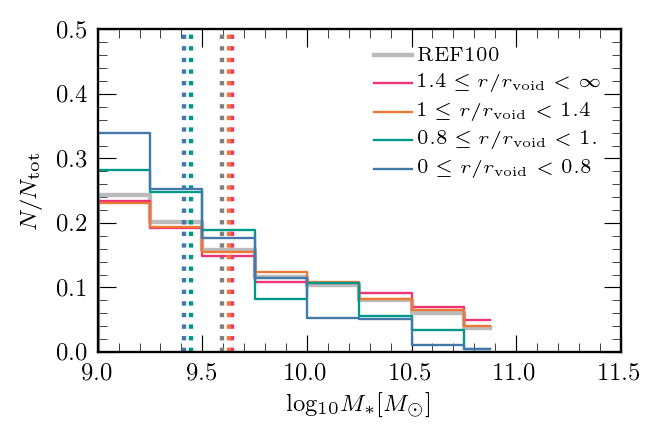
\includegraphics[width=1\columnwidth]{plots_parent_sample/GMF_cs_three_regions.png} &
	
%	\includegraphics[width=1\columnwidth]{plots_halo_starmass_centrals/u_r_fraction_threeregions.png} & 
	%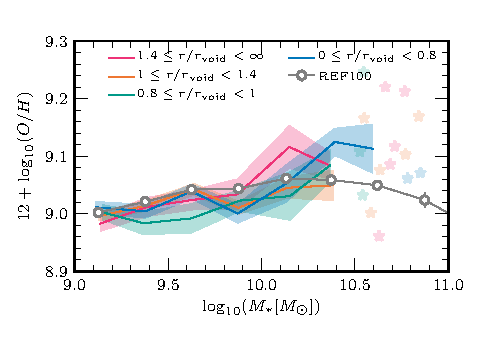
\includegraphics[width=1\columnwidth]{plots_halo_starmass_centrals/mass_metallicity_threeregions_v1.pdf} \\
	%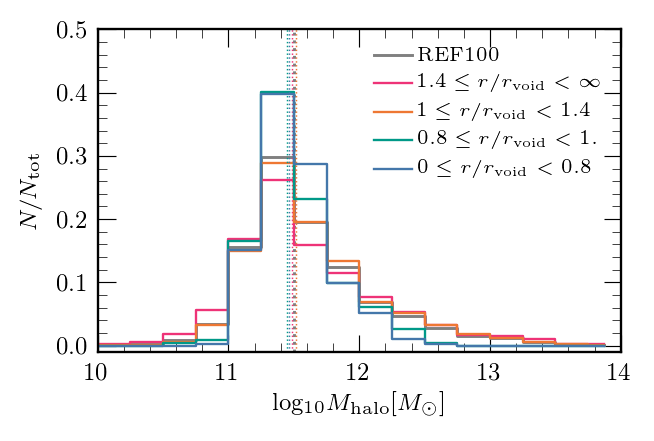
\includegraphics[width=0.95\columnwidth]{plots_parent_sample/HMF_cs_three_regions.png} &
 	%\includegraphics[width=1\columnwidth]{plots_halo_starmass_centrals/mass_ssfr_threeregions.pdf} &

	%\includegraphics[width=1\columnwidth]{plots_halo_starmass_centrals/mass_sizes_threeregions_stars.pdf} \\
	%\end{tabular}	
    %\caption{Galaxy properties of the sub-samples from outer void, wall and skeleton galaxies that are defined by the void centric distance as the legend indicates: outer void (green), wall (orange) and skeleton (magenta) galaxies. These subsamples were selected such as they have the same stellar mass and halo mass distribution as the parent sample of inner void galaxies. Grey colour represents all the central galaxies in the simulation. \textit{Top left panel:} Distribution of u-r for each sub-sample and the galaxy parent sample of inner voids. \textit{ Top right panel:} The mean relation between stellar mass  and the star forming gas-phase  oxygen abundance.  Shaded regions represent the error of the mean of each sample and diffused markers correspond to galaxies in bins with less than 5 galaxies. \textit{ Bottom left panel:} The mean specific star formation rate (sSFR) as a function of the stellar mass. Coloured marker and solid lines represent the mean distribution and error bars represent the error of the mean. Diffused  stars correspond to galaxies in stellar mass bins with less than 5 galaxies. Grey contours and the diffuse density map represent all the central star forming  galaxies in the simulation. \textit{Bottom right panel:} The mean half-stellar mass radius as a function of stellar mass for each galaxy sub-sample sample. Error bars correspond to the error of the mean and grey markers for all the simulation. Diffused markers correspond to observation data from  Fernandez-Lorenzo et al.2013. }
%    \label{fig:ssmhm}
%\end{figure*}





\subsection{Properties of central disc galaxies}

The study of metallicity in galaxies have revealed that metals are distributed in-homogeneously throughout  galaxies, exhibiting  metallicity gradients from which we could decipher the mechanisms that  redistribute  gas  such as  torques driven by bars or inflows driven by SN and AGN feedback.  Mergers and interactions can also contribute by modifying the gas properties and  mixing chemical elements and triggering strong star formation activity. 

In this section, we will focus on  the impact of the large-scale environment  on the re-distribution of gas, in particular, the gas-phase oxygen abundance gradients. We concentrate our study in disc  galaxies, which has been observed with steep gradients. We study only massive disc galaxies that have enough stellar particles to accurately resolve the disc and its internal structure ( $M_{*}\geq 10^{10}\Msun$ with more than $10^4$ particles).  For inner void galaxies, we have 10 massive discs whereas  26, 391 and  165 discs  are found in outer void, wall and skeleton galaxies respectively. These fractions are pretty low but it is still worth to mention the general differences in their properties as a function of the distance to the closest void centre. 


Fig.~\ref{fig:discs} presents  the cumulative age distribution of the youngest (30 per cent) of the stellar population (left panel) for the parent samples of inner void (blue), outer void (green),  wall (orange) and skeleton (magenta) massive disc galaxies. From the figure, it is clear than more than 40 per cent of inner void galaxies,  their youngest population  was born during the last 3 Gyrs ago while the youngest population of above 80 per cent of outer void, wall and skeleton galaxies already was born. This is consistent with the  low efficiency of gas converting into stars  in inner void galaxies combined with their  quiet major and minor merger histories in comparison with those from skeleton and wall galaxies (see section~\ref{subsubsec:MHs}).  

The massive discs population in the simulation \REF~ has been explored by \cite{tissera2019}. Particularly, the authors find a large diversity of  gas-phase oxygen  gradients with $~ 40$ per cent of them  to be positive. Positive gradients could be caused by external and internal processes in the disc galaxies. Interactions with other galaxies have been pointed as an external process  whereas, torques driven by stellar bars and inflows from AGN and SN feedback to be secular processes that could redistribute the gas in disc galaxies. 
\cite{tissera2019} found that  massive disc galaxies in EAGLE tend to have a shallower relation between gas-phase oxygen abundances gradients and  stellar mass  probably because they have a higher probability of experiencing mergers and to be located in higher density regions. The right panel of  Fig.~\ref{fig:discs} shows the distribution of the gas-phase oxygen abundances gradients for the four parent samples.   The gas-phase oxygen abundances gradients  are  calculated in  \citet{tissera2019} by fitting a linear regression to the abundance profiles on the disc plane, in the radial interval [0.5,1.5]$R_{\rm eff}$ where $R_{\rm eff}$ is the radius that encloses 50 per cent of the stellar mass of the disc.  From the figure is clear that  inner void massive discs present the most negative gas-phase oxygen abundances gradients ($~ 40$ per cent) with a mean value of $-0.028\, \rm dex kpc^{-1}$. In comparison, the rest of the subsamples present a similar distribution of gas-phase oxygen abundances gradients with mean values of $0.006,-0.011,-0.011\, \rm dex kpc^{-1}$ for outer void, wall and skeleton galaxies.  \textcolor{green}{Nelson: this section is great!  Is this with controlled stellar mass?}



\begin{figure*}	
	% To include a figure from a file named example.*
	% Allowable file formats are eps or ps if compiling using latex
	% or pdf, png, jpg if compiling using pdflatex
    \begin{tabular}{cc}
	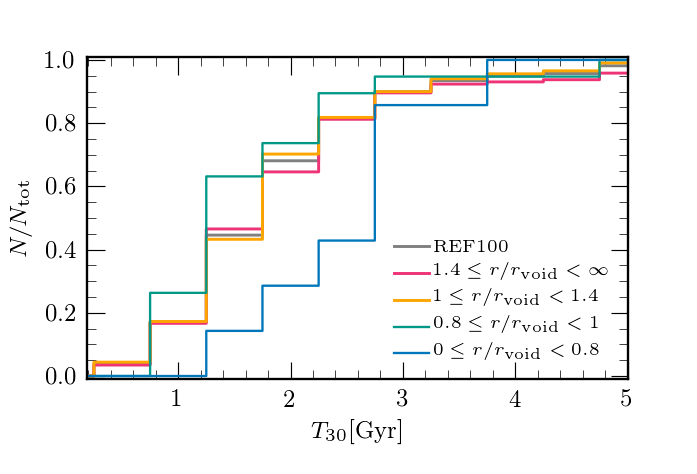
\includegraphics[width=1\columnwidth]{plots_parent_sample/T30_fraction_threeregionscum.png} &
	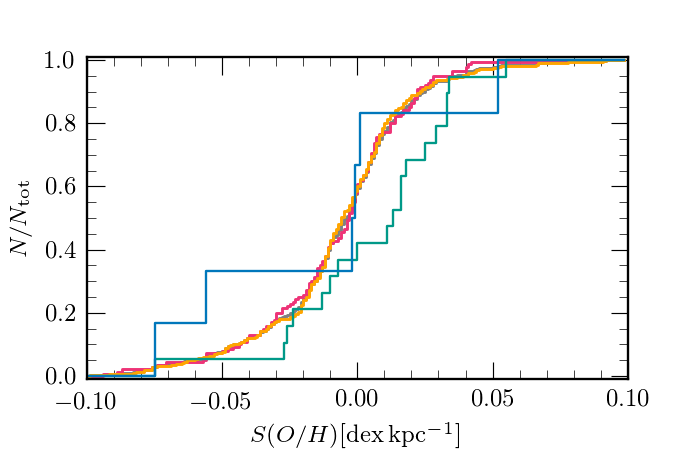
\includegraphics[width=1\columnwidth]{plots_parent_sample/SOH_fraction_threeregionscum.png} \\
	\end{tabular}
    \caption{\textit{ Left panel:} The cumulative  age distribution  of the youngest 30 per cent of the stellar population in massive discs ($M_{*}\geq 10^{10}\Msun$) of inner void, outer void, wall and skeleton galaxies. Massive discs in inner void galaxies present older stellar populations than the rest of the galaxies.\textit{Right panel:} The cumulative  gas-phase oxygen abundance distribution in massive star forming discs of inner void, outer void, wall and skeleton galaxies. More than 40 per cent of inner void galaxies present the most negative  oxygen abundance gradients.}    \label{fig:discs}
\end{figure*}





\section{ Summary and Discussion}
In this paper, we investigate the properties galaxies as a function of the closest void centre using a  $\Lambda$CDM  cosmological hydrodynamical simulation \REF from the EAGLE project.  The simulation evolves a comoving region of 100 $\rm cMpc$ on a side with  an initial number of  DM and gas  particles  of $2\times 1570^3$ and does so with a model for galaxy formation physics which reasonably reproduces  many galaxy observables \citep{schaye2015,crain2015,furlong2015}.  
The resolution of the simulation allows the effects of large-scale environment in a cosmological context. Our study concentrate in central galaxies with a stellar mass larger than $10^9 \Msun$ that results in 7400 central galaxies. To identified voids in the simulation, we  work with the void catalogue constructed in \cite*{paillas2017} by using a spherical under-density finder \citep{padilla2005}. The void catalogue consists in 709 voids with 9 of them with $\Rvoid$ larger than $10\pMpc$ and the smallest void with a radius above $3\pMpc$. 
For each galaxy, we calculate the .....  
 

OJO, only comments of Patricia to Yetli. Conclusions will be included soon
1. By selecting galaxies in the four defined regions to have the consistent stellar mass distribution to the inner halo galaxies,
we found that:
i) the median O/H of the gas-phase is systematically lower in lower regions, except for galaxies with $M > 10.5$.
ii) The colour bimodality is only present near the walls and skeletons but within the void the distribution of colour is uni-modal.
iii) No differences in galaxy sizes are found .
iv) ssfr no se puede ver bien .

2. By selecting galaxies to have both similar stellar mass distribution and dark matter halo distributions we are left with smaller
dark matter haloes.
i) the colour distributions are similar and unimodal, even if the range of masses are similar; the red peak is associated to the larger impact of
environment defined by more massive dark matter haloes.
ii) there is not clear difference in the chemical abundances except for the most massive galaxies that tend to have higher levels near the wall.
iii) Massive galaxies en la figura 4 size-mass no hay  para los azuloes  pero si estan cuando se mira oh.??
iv) sSFr el mismo problema de antes

3. central galaxies with similar stellar mass distribution (and dark matter??? no clear).
The distributions get noisier and I am not quite sure of the trends

4. Fig.6: I donot follow from which subsample are taken, those of fig. 5 (central galaxies with similar stellar mass and dark matter distributions??).
$M>10^10\Msun$
i) disc galaxies in the inner void have less active star formation than galaxies in the walls and skeletons and they have more negative metallicity gradients.
This suggests that galaxies in the inner void have evolved more quiescently and  passively, compared to galaxies in the skeletons and walls.
The latter are consistent with more continuous gas accretion which can be linked to higher star formation activities (left panel) and flatter metallicity gradients.

~                                                                                      


\section*{Acknowledgements}

The Acknowledgements section is not numbered. Here you can thank helpful
colleagues, acknowledge funding agencies, telescopes and facilities used etc.
Try to keep it short.

%%%%%%%%%%%%%%%%%%%%%%%%%%%%%%%%%%%%%%%%%%%%%%%%%%

%%%%%%%%%%%%%%%%%%%% REFERENCES %%%%%%%%%%%%%%%%%%

% The best way to enter references is to use BibTeX:

%\bibliographystyle{mnras}
%\bibliography{example} % if your bibtex file is called example.bib


% Alternatively you could enter them by hand, like this:
% This method is tedious and prone to error if you have lots of references
%\begin{thebibliography}{99}
%\bibitem[\protect\citeauthoryear{Author}{2012}]{Author2012}
%Author A.~N., 2013, Journal of Improbable Astronomy, 1, 1
%\%bibitem[\protect\citeauthoryear{Others}{2013}]{Others2013}
%Others S., 2012, Journal of Interesting Stuff, 17, 198


\begin{thebibliography}{99}
\bibitem [\protect\astroncite{Abramowicz et al.}{1995}]{abramowicz1995} 
{Abramowicz}, M.~A. , {Chen}, X. , {Taam}, R.~E., 1995, ApJ, 452, 379.

\bibitem [\protect\astroncite{Aird et al.}{2010}]{aird2010} 
{Aird}, J. , {Nandra}, K. , {Laird}, E.~S. and {Georgakakis}, A. , 
{Ashby}, M.~L.~N. , {Barmby}, P. , {Coil}, A.~L. , {Huang}, J.-S. , 
{Koekemoer}, A.~M. , {Steidel}, C.~C. and {Willmer}, C.~N.~A.
2010, MNRAS, 401, 2531.

\bibitem [\protect\astroncite{Aird et al.}{2015}]{aird2015} 
Aird, J., Coil, A.~L., Georgakakis, A., et al.\ 2015, arXiv:1503.01120

\bibitem [\protect\astroncite{Angles-Alcazar et al.}{2016}]{angles-alcazar2016}
Angl{\'e}s-Alc{\'a}zar, D., Dav{\'e}, R., Faucher-Gigu{\`e}re, C.-A., {\"O}zel, F., \& Hopkins, P.~F,, 2016, arXiv:1603.08007 

\bibitem[\protect\astroncite{Bah{\'e} et al.}{2016}]{bahe2016} 
Bah{\'e}, Y.~M., Crain, R.~A., Kauffmann, G., et al.\ 2016, \mnras, 456, 1115 
 
 \bibitem[\protect\citeauthoryear{Baldry, et al.}{2012}]{baldry2012} 
 Baldry I.~K., et al., 2012, MNRAS, 421, 621

\bibitem[\protect\astroncite{Bandara et al.}{2009}]{bandara2009} 
Bandara,~K., Crampton,~D., Simard, ~L., 2009, ApJ, 704, 1135. 

\bibitem[\protect\astroncite{Binney \& Tabor}{1995}]{binney_tabor1995} 
Binney J., Tabor G., 1995, MNRAS, 276, 663. 

\bibitem[\protect\astroncite{Bondi \& Hoyle}{1944}]{bondi44} 
Bondi ~H., Hoyle ~F., 1944, MNRAS, 104, 273.

\bibitem[\protect\astroncite{Booth \& Schaye}{2009}]{booth_schaye2009} 
Booth C.~M., Schaye ~J., 2009, MNRAS, 398, 53.

\bibitem[\protect\astroncite{Booth \& Schaye}{2010}]{booth_schaye2010} 
Booth C.~M., Schaye ~J., 2010, MNRAS, 405, L1.




\bibitem[\protect\astroncite{Bower et al.}{2006}]{bower2006} Bower R.~G.,
Benson A.~J., Malbon R., Helly J.~C., Frenk C.~S., Baugh C.~M., Cole S., Lacey
C.~G., 2006, MNRAS, 370, 645. 



\bibitem[\protect\astroncite{Buchner et al.}{2015}]{buchner2015} 
Buchner J., Georgakakis A., Nandra K., et al. 2015, ApJ, 802, 89. 


\bibitem[\protect\astroncite{Chabrier}{2003}]{chabrier2003} 
Chabrier, G., 2003, PASP, 115, 763.

\bibitem[\protect\astroncite{Choi et al.}{2013}]{choi2013} 
Choi, E., Naab, T., Ostriker, J.~P., Johansson, P.~H., \& Moster, B.~P., 2014, MNRAS, 442, 440.

\bibitem[\protect\astroncite{Churazov et al.}{2001}]{churazov2001} 
Churazov E., Br{\"u}ggen M., Kaiser C.~R., B{\"o}hringer H., Forman W., 2001, ApJ, 554, 261. 

\bibitem[\protect\astroncite{Comerford et al.}{2014}]{comerford2014}
Comerford, J.~M., \& Greene, J.~E.\ 2014, ApJ, 789, 112 



\bibitem[\protect\astroncite{Comerford et al.}{2015}]{comerford2015}
Comerford, J.~M., Pooley, D., Barrows, R.~S., et al.\ 2015, ApJ, 806, 219 

\bibitem[\protect\astroncite{Crain et al.}{2009}]{crain09}
Crain R.~A., Theuns ~T., Dalla Vecchia ~C., Eke V.~R. , Frenk S.~C., Jenkins ~A., Kay S.~T. and Peacock J.~A. {\it et al.}, 2009, MNRAS,  399, 1773.

\bibitem[\protect\astroncite{Crain et al.}{2015}]{crain2015}
Crain, R.~A., Schaye, J., Bower, R.~G., et al.\ 2015, arXiv:1501.01311 

\bibitem[\protect\astroncite{Croton et al.}{2006}]{croton2006}
Croton D. ~J., Springel V., White S. ~D. ~M., De Lucia ~G., Frenk S. C., Gao L., Jenkins ~A. and Kauffmann ~G. {\it et al.}, 2006, MNRAS, 365, 11.

\bibitem[\protect\astroncite{Cullen \& Dehnen}{2010}]{cullen_dehnen2010} 
Cullen, L. and Dehnen, W., 2010, MNRAS, 408, 669.  


\bibitem[\protect\astroncite{Dalla Vecchia \& Schaye}{2012}]{dallavecchia_schaye12} 
Dalla Vecchia  ~C. and Schaye ~J., 2012, MNRAS, 426, 140.




\bibitem[\protect\astroncite{De Lucia \& Blaizot}{2007}]{delucia2007} 
De Lucia G., Blaizot J., 2007, MNRAS, 375, 2


\bibitem[\protect\astroncite{Di Matteo et al.}{2008}]{dimatteo2008}
Di Matteo, T. and Colberg, J. and Springel, V. and Hernquist, L. and  Sijacki, D., 2008, ApJ, 676, 33.

\bibitem[\protect\astroncite{Dolag et al}{2009}]{dolag2009} 
Dolag K., Borgani S., Murante G., Springel V., 2009, MNRAS,399, 497

\bibitem[\protect\astroncite{Done et al.}{2007}]{done2007} 
Done, C., Gierli{\'n}ski, M., \& Kubota, A.\ 2007, A\&ARv, 15, 1

\bibitem[\protect\astroncite{Durier \& Dalla Vecchia}{2012}]{durier_dallavecchia12} 
Durier, F. and Vecchia D.~C., 2012, MNRAS, 419, 465.



\bibitem[\protect\astroncite{Fanidakis et al.}{2012}]{fanidakis12}
 {Fanidakis} N. and {Baugh} C.~M. and {Benson} A.~J. and {Bower} R.~G. and 
{Cole} S. and {Done} C. and {Frenk} C.~S. and {Hickox} R.~C. and 
{Lacey} C. and {Del P.~Lagos} C., 2012, MNRAS, 419, 2797.


 
\bibitem[\protect\astroncite{Ferland et al.}{2013}]{ferland2013} 
G. J. Ferland, R. L. Porter, P. A. M. van Hoof, R. J. R. Williams, N. P. Abel, M. L. Lykins, Gargi Shaw, W. J. Henney, and P. C. Stancil, 2013, Rev. Mex. Soc., 49, 1.

\bibitem[\protect\citeauthoryear{Fern{\'a}ndez Lorenzo, et al.}{2013}]{fernandez-lorenzo2013} Fern{\'a}ndez Lorenzo M., Sulentic J., Verdes-Montenegro L., Argudo-Fern{\'a}ndez M., 2013, MNRAS, 434, 325



\bibitem[\protect\astroncite{Furlong et al.}{2015a}]{furlong2015a}
Furlong, M., Bower, R.~G., Theuns, T., et al.\ 2015, MNRAS, 450, 4486   

\bibitem[\protect\astroncite{Furlong et al.}{2015b}]{furlong2015b}
Furlong, M., Bower, R.~G., Crain, R.~A., et al.\ 2015, arXiv:1510.05645

\bibitem[\protect\astroncite{Giallongo et al.}{2015}]{giallongo2015} 
Giallongo, E., Grazian, A., Fiore, F., et al., 2015, AAP, 578, A83

\bibitem[\protect\astroncite{Graham}{2016}]{graham2016} 
Graham, A.~W., 2016, Galactic Bulges, 418, 263 

\bibitem[\protect\astroncite{Grogin et al.}{2011}]{grogin2011} 
Grogin, N. A., Kocevski, D., Faber, S. et al. 2011, ApJS, 197, 37





\bibitem[\protect\astroncite{Haardt \& Madau.}{2001}]{haardt2001} 
{Haardt}, F. and {Madau}, P., 2001, Clusters of Galaxies and the High Redshift Universe Observed in X-rays, 
astro-ph/0106018. 


\bibitem[\protect\astroncite{Hasinger et al.}{2005}]{hasinger2005}
{Hasinger}, G. and {Miyaji}, T. and {Schmidt}, M., 2005, A\&A, 441, 417.

\bibitem[\protect\astroncite{Hasinger}{2008}]{hasinger2008}
{Hasinger}, G., 2008, A\& A, 490, 905.


\bibitem[\protect\astroncite{Hirschmann et al.}{2014}]{hirschmann2014}
Hirschmann, M., Dolag, K., Saro, A., et al.\ 2014, MNRAS, 442, 2304 


\bibitem[\protect\astroncite{Hirschmann et al.}{2012}]{hirschmann2012}
{Hirschmann} M.,  {Somerville} R.~S.,  {Naab} T.,    {Burkert} A.,  2012,
  MNRAS, 426, 237



\bibitem[\protect\astroncite{Hopkins et al.}{2007}]{hopkins2007}  
Hopkins, P.~F.,  Richards, G.~T., \& Hernquist, L., 2007, ApJ, 654, 731 

\bibitem[\protect\astroncite{Hopkins et al.}{2009}]{hopkins2009}  
{Hopkins} P.~F., and {Hernquist} L.,  {Cox} T.~J. , {Keres} D. and 
{Wuyts} S., 2009, ApJ, 691, 1424.


\bibitem[\protect\astroncite{Jenkins}{2010}] {jenkins2010}
Jenkins ~A., 2010, MNRAS, 403, 1859.

\bibitem[\protect\astroncite{Jenkins}{2013}] {jenkins2013}
Jenkins ~A., 2013, MNRAS, 434, 2094.



\bibitem[\protect\astroncite{Kelly \&  Shen}{2013}]{kelly2013}
Kelly B.~C.,  Shen Y.,  2013, ApJ, 764, 45.




\bibitem[\protect\astroncite{Kennicutt}{1998}] {kennicut1998}
Kennicutt, Jr., R. C., 1998, ARA\&A, 36, 189.

\bibitem[\protect\astroncite{Khandai et al.}{2015}]{khandai2015} 
Khandai, N. and Di Matteo, T. and Croft, R. and Wilkins, S.~M. and 
	Feng, Y. and Tucker, E. and DeGraf, C. and Liu, M.-S., 2015,
MNRAS, 450, 1349 

\bibitem[\protect\astroncite{Koekemoer et al.}{2011}]{koekemoer2011} 
Koekemoer, A. M., Faber, S., Ferguson, H. et al. 2011, ApJS, 197, 36



\bibitem[\protect\astroncite{Kormendy \& Ho }{2013}]{kormendy_ho2013} 
Kormendy, J. and Ho, L.~C., 2013, ARA\&A ,51,511.

\bibitem[\protect\astroncite{Koss et al. }{2012}]{koss2012} 
Koss, M., Mushotzky, R., Treister, E., et al.\ 2012, ApJl, 746, L22 

\bibitem[\protect\astroncite{Lagos et al.}{2015}]{lagos2015}
Lagos, C.~d.~P., Crain, R.~A., Schaye, J., et al., 2015, arXiv:1503.04807

\bibitem[\protect\astroncite{Lansbury et al.}{2015}]{lansbury2015}
Lansbury, G.~B., Gandhi, P., Alexander, D.~M., et al., 2015, ApJ, 809, 115 

\bibitem[\protect\astroncite{Lewis et al.}{2000}]{lewis2000}
Lewis A., Challinor A., Lasenby A., 2000, ApJ, 538, 473

\bibitem[\protect\astroncite{Liu et al.}{2011}]{liu2011}
Liu, X., Shen, Y., Strauss, M.~A., \& Hao, L.\ 2011, ApJ, 737, 101 


\bibitem[\protect\astroncite{Lusso et al.}{2012}]{lusso2012} 
Lusso, E., Comastri, A., Simmons, B.~D., et al., 2012, MNRAS, 425, 623 

 
\bibitem[\protect\astroncite{Madau \& Haardt.}{2015}]{madau2015} 
Madau, P., \& Haardt, F., 2015, ApJ, 813, L8 


\bibitem[\protect\astroncite{Marconi et al.}{2004}]{marconi2004} 
{Marconi}, A. and {Risaliti}, G. and {Gilli}, R. and {Hunt}, L.~K. and 
{Maiolino}, R. and {Salvati}, M., 2004, MNRAS, 351, 169.   


\bibitem[\protect\astroncite{McAlpine et al.}{2015}]{mcAlpine2015} 
McAlpine S., Helly J.C., Schaller M., et al.\ 2015, arXiv:1510.01320

\bibitem[\protect\astroncite{McCarthy et al.}{2010}]{mcCarthy2010} 
McCarthy  I.~G., Schaye ~J., Ponman T.~J., Bower R.~G., Booth C.~M., Dalla Vecchia C., Crain R.~A. and Springel V.,
2010, MNRAS,  406, 822.


\bibitem[\protect\astroncite{McConnell \& Ma}{2013}]{mcConnell_ma2013} 
McConnell, N.~J., \& Ma, C.-P., 2013, ApJ, 764, 184 



\bibitem[\protect\astroncite{Miyaji et al.}{2000}]{miyaji2000}
{Miyaji} T.,  {Hasinger} G., {Schmidt} M.,  2000, A\&A, 353, 25.


\bibitem[\protect\astroncite{Miyaji et al.}{2015}]{miyaji2015}
Miyaji, T., Hasinger, G., Salvato, M., et al., 2015, ApJ, 804, 104


\bibitem[\protect\astroncite{Narayan \& Yi}{1994}]{narayan_yi1994}
{Narayan}, R. and {Yi}, I., 1994,  ApJ, 428, L13.
\bibitem[\protect\citeauthoryear{Padilla et al.}{2005}]{padilla2005} 
Padilla N.~D., Ceccarelli L., Lambas D.~G., 2005, MNRAS, 363, 977

\bibitem[\protect\citeauthoryear{Paillas et al.}{2017}]{paillas2017} 
Paillas E., Lagos C.~D.~P., Padilla N., Tissera P., Helly J., Schaller M., 2017, MNRAS, 470, 4434


\bibitem[\protect\astroncite{Planck collaboration et al.}{2013}]{planck13} 
{Planck Collaboration} and {Ade}, P.~A.~R. and {Aghanim}, N. and 
	{Alves}, M.~I.~R. and {Armitage-Caplan}, C. and {Arnaud}, M. and 
	{Ashdown}, M. and {Atrio-Barandela}, F. and {Aumont}, J. and 
	{Aussel}, H. and et al., 2013, arxiv e-prints, 1303.5062.

\bibitem[\protect\astroncite{Portinari et al.}{1998}]{portinari1998} 
Portinari L., Chiosi C., \& Bressan A.\ 1998, A\& A, 334, 505.  


\bibitem[\protect\astroncite{Power et al.}{2010}]{power2011} Power, C. and
Nayakshin, S. and King, A., 2011, MNRAS, 412, 269.


\bibitem[\protect\astroncite{Rees et al.}{1982}]{rees1982}
Rees, M.~J. and Begelman, M.~C. and Blandford, R.~D. and 
Phinney, E.~S., 1982, NATURE, 295, 17.

\bibitem[\protect\citeauthoryear{Ricciardelli, et al.}{2014}]{ricciardelli2014} Ricciardelli E., Cava A., Varela J., Quilis V., 2014, MNRAS, 445, 4045


\bibitem[\protect\astroncite{Rosas-Guevara et al.}{2015}]{rosas-guevara2015}
Rosas-Guevara Y. M., Bower R.G., Schaye J., et al.\ 2015, MNRAS, 454, 1038 

\bibitem[\protect\astroncite{Rosas-Guevara et al.}{2016}]{rosas-guevara2016}
Rosas-Guevara, Y., Bower, R.~G., Schaye, J., et al.\ 2016, MNRAS, 462, 190
\bibitem[\protect\astroncite{Shakura \& Syunyaev}{1973}]{shak73} 
Shakura N.I ., Syunyaev R. A., 1973, A\&A , 24, 337.

\bibitem[\protect\astroncite{Schaller et al.}{2015}]{schaller2015}
Schaller, M., Dalla Vecchia, C., Schaye, J., et al., 2015, MNRAS, 454, 2277


\bibitem[\protect\astroncite{Schaye}{2004}]{schaye2004} 
Schaye, J., 2004, ApJ, 609, 667 


\bibitem[\protect\astroncite{Schaye \& Dalla Vecchia}{2008}]{scha08} 
Schaye J., Dalla Vechia C., 2008, MNRAS, 383, 1210.

\bibitem[\protect\astroncite{Schaye et al.}{2010}]{scha10} 
Schaye ~J., Dalla Vecchia ~C., Booth C.~M., Wiersma R.~P.~C., Theuns ~T., Haas M.~R., Bertone ~S. and Duffy A.~R.{\it et al.},
 2010, MNRAS, 402, 1536. 


\bibitem[\protect\citeauthoryear{Schaye et al.}{2015}]{schaye2015} 
Schaye, J., Crain, R.~A., Bower, R.~G., et al.\ 2015, MNRAS, 446, 521 

\bibitem[\protect\citeauthoryear{Shen, et al.}{2003}]{shen2003} 
Shen S., et al., 2003, MNRAS, 343, 978


\bibitem[\protect\astroncite{Schmidt}{1959}]{schmidt1959} 
Schmidt, M., 1959, ApJ, 129, 243.

 

\bibitem[\protect\astroncite{Shankar et al.}{2004}]{shankar2004} 
{Shankar}, F. and {Salucci}, P. and {Granato}, G.~L. and {De Zotti}, G. and 
{Danese}, L., 2004, MNRAS, 354, 1020.


\bibitem[\protect\astroncite{Shankar et al.}{2013}]{shankar2013} 
Shankar, F., 2013, Classical and Quantum Gravity, 30, 244001

\bibitem[\protect\astroncite{Sijacki et al.}{2007}]{sijacki2007} 
Sijacki ~D., Springel ~V., Di Matteo ~T. and Hernquist ~L., 2007
MNRAS,  380, 877.

\bibitem[\protect\astroncite{Sijacki et al.}{2015}]{sijacki2015} 
Sijacki, D., Vogelsberger, M., Genel, S., et al.\ 2015, MNRAS, 452, 575 


\bibitem[\protect\astroncite{Soltan}{1982}]{soltan1982} 
Soltan ~A., 1982, MNRAS, 200, 115.

\bibitem[\protect\astroncite{Springel et al.}{2001}]{springel2001}
Springel V., White S. D. M., Tormen G., Kau?mann G.,2001, MNRAS, 328, 726



\bibitem[\protect\astroncite{Springel et al.}{2005a}]{springel2005a}
Springel ~V., Di Matteo ~T. and Hernquist ~L., 2005,
MNRAS, 361, 776.

\bibitem[\protect\astroncite{Springel}{2005b}]{springel2005b}
Springel, ~V., 2005b, MNRAS, 364, 1105.

\bibitem[\protect\astroncite{Steffen et al.}{2003}]{steffen2003}
{Steffen}, A.~T. and {Barger}, A.~J. and {Cowie}, L.~L. and 
	{Mushotzky}, R.~F. and {Yang}, Y., 2003, ApJ, 596, L23.

\bibitem[\protect\astroncite{Steinborn et al.}{2016}]{steinborn2016}
Steinborn, L.~K., Dolag, K., Comerford, J.~M., et al.\ 2016, MNRAS, 458, 1013 


\bibitem[\protect\astroncite{Trayford et al.}{2016}]{trayford2016} 
Trayford, J.~W., Theuns, T., Bower, R.~G., et al.\ 2016, arXiv:1601.07907 

\bibitem[\protect\citeauthoryear{Tissera, et al.}{2019}]{tissera2019} 
Tissera P.~B., et al., 2019, MNRAS, 482, 2208

\bibitem[\protect\astroncite{Tremaine et al.}{2002}]{tremaine2002} 
Tremaine ~S., Gebhardt ~K., Bender ~R., Bower ~G., Dressler ~A., Faber S. ~M., Filippenko A. ~V. and Green ~R. {\it et al.},
2002, ApJ, 574, 740.


\bibitem[\protect\astroncite{Treister et al.}{2009}]{treister2009} 
Treister, E., Urry, C. M., \& Virani, S., 2009, ApJ, 696, 110

\bibitem[\protect\astroncite{Ueda et al.}{2003}]{ueda2003} 
{Ueda}, Y. and {Akiyama}, M. and {Ohta}, K. and {Miyaji}, T.,
2003,ApJ , 598, 886.

\bibitem[\protect\astroncite{Ueda et al.}{2014}]{ueda2014}
 Ueda, Y., Akiyama, M., Hasinger, G., Miyaji, T., \& Watson, M.~G.\ 2014, ApJ, 786, 104 

 





\bibitem[\protect\astroncite{Vasudevan \& Fabian}{2009}]{vasudevan2009} 
Vasudevan R. V., Fabian A. C., 2009, MNRAS, 392, 1124

\bibitem[\protect\astroncite{Vogelsberger et al.}{2014}]{vogelsberger2014} 
Vogelsberger, M., Genel, S., Springel, V., et al., 2014, MNRAS, 444, 1518

\bibitem[\protect\astroncite{Volonteri et al.}{2016}]{volonteri2016} 
Volonteri, M., Dubois, Y., Pichon, C., \& Devriendt, J.\ 2016, MNRAS, 460, 2979


\bibitem[\protect\astroncite{ Yu \& Tremaine}{2002}]{yu_tremaine_2002}
{Yu}, Q. and {Tremaine}, S., 2002, MNRAS, 335, 965.



\bibitem[\protect\astroncite{Wiersma et al.}{2009a}]{wiersma2009a}
Wiersma R.~P.~C., Schaye ~J., Theuns ~T., Smith B.~D,
2009,  MNRAS, 393, 99.

\bibitem[\protect\astroncite{Wiersma et al.}{2009b}]{wiersma2009b}
Wiersma R.~P.~C., Schaye ~J., Theuns ~T., Dalla Vecchia ~C. and Tornatore ~L.,
2009,  MNRAS, 399, 574.


\end{thebibliography}

%%%%%%%%%%%%%%%%%%%%%%%%%%%%%%%%%%%%%%%%%%%%%%%%%%

%%%%%%%%%%%%%%%%% APPENDICES %%%%%%%%%%%%%%%%%%%%%

%%\appendix

%%\section{Convergence tests}
%%Varying parameters and  also definition of active AGN. 
%\section{Evolution of Luminosity of AGN binaries in small scales }

%%\begin{figure}
	% To include a figure from a file named example.*
	% Allowable file formats are eps or ps if compiling using latex
	% or pdf, png, jpg if compiling using pdflatex
	%\includegraphics[width=1.1\columnwidth]{plots/evolutionBHB_8203962953467_8185581101601.png}
    %\caption{.}
    %\label{fig:apendx}
%\end{figure}

%\begin{figure}
	% To include a figure from a file named example.*
	% Allowable file formats are eps or ps if compiling using latex
	% or pdf, png, jpg if compiling using pdflatex
	%\includegraphics[width=1.1\columnwidth]{plots/evolutionBHB_8330790016083_8324985796263.png}
    %\caption{.}
    %\label{fig:apendx}
%\end{figure}


%\begin{figure}
	% To include a figure from a file named example.*
	% Allowable file formats are eps or ps if compiling using latex
	% or pdf, png, jpg if compiling using pdflatex
	%\includegraphics[width=1.1\columnwidth]{plots/evolutionBHB_8547583296243_8633372065199.png}
    %\caption{.}
    %\label{fig:apendx}
%\end{figure}




%\begin{figure}
	% To include a figure from a file named example.*
	% Allowable file formats are eps or ps if compiling using latex
	% or pdf, png, jpg if compiling using pdflatex
	%\includegraphics[width=1.1\columnwidth]{plots/evolutionBHB_1877078178159_1878852559925.png}
    %\caption{.}
    %\label{fig:apendx}
%\end{figure}

%\begin{figure}
	% To include a figure from a file named example.*
	% Allowable file formats are eps or ps if compiling using latex
	% or pdf, png, jpg if compiling using pdflatex
	%\includegraphics[width=1.1\columnwidth]{plots/evolutionBHB_2870834935551_2871017060413.png}
    %\caption{.}
    %\label{fig:apendx}
%\end{figure}


%\begin{figure}
	% To include a figure from a file named example.*
	% Allowable file formats are eps or ps if compiling using latex
	% or pdf, png, jpg if compiling using pdflatex
	%\includegraphics[width=1.1\columnwidth]{plots/evolutionBHB_2889262306783_1518874155979.png}
    %\caption{.}
    %\label{fig:apendx}
%\end{figure}



%%%%%%%%%%%%%%%%%%%%%%%%%%%%%%%%%%%%%%%%%%%%%%%%%%


% Don't change these lines
\bsp	% typesetting comment
\label{lastpage}
\end{document}

% End of mnras_template.tex